\documentclass[10pt]{article}
\usepackage[margin=1in]{geometry}
\usepackage{epsfig}
\usepackage{float}
\usepackage{subfigure}
\usepackage{algorithm}
\usepackage{algorithmic}
\def\ert{\mbox{{\it expRunTime}}}
\def\sertput{\mbox{{\it sendExpRunTimeToPUT}}}
\def\rpe{\mbox{{\it recordPUTExecution}}}
\def\procDiff{\mbox{{\it procDiff}}}
\def\getProcDiff{\mbox{{\it getProcDiff}}}
\def\bfps{\mbox{{\it beforeProcs}}}
\def\afps{\mbox{{\it afterProcs}}}
\def\gpi{\mbox{{\it getProcInfo}}}
\def\ect{\mbox{{\it elapsedClockTime}}}
\def\pt{\mbox{{\it ProgramTime}}}
\def\cpt{\mbox{{\it computeProgramTime}}}
\long\def\shorten#1{}
\begin{document}
\title{Characterization of Program Execution Time Distribution}

\author{
Young-Kyoon Suh\\
Department of Computer Science \\
University of Arizona \\
\small\tt \{yksuh\}@cs.arizona.edu
}
\maketitle

\section{Observed Phenomena}
In this section, we discuss interesting phenomena observed from our measurements on 
a program-under-test (PUT) with a given task length. 
PUT is a simple compute-only program that runs a nested-for loop for a given amount of time (task length) and terminates.

%For instance, PUT8 denotes PUT taking 8 seconds as its task length. 
%In this report, we use two types of program execution time: elapsed time (ET) and program time (PT). 
%ET is computed as the difference of the wall-clock times measured before and after PUT execution.
%PT is calculated as the sum of the user time and system time of PUT. 

\subsection{Different Bands in Elapsed Time}
\label{sec:bands}

We introduce an interesting phenomenon regarding the elapsed time (ET) of PUT.
ET is computed as the difference of the wall-clock times measured before and after PUT execution.

\paragraph{Presumption} Little structure in ET

\paragraph{Description} Figure~\ref{fig:et_plot} shows the distribution of ET on PUT16 and PUT32. 
In this report, PUT$x$ denotes the PUT with $x$-second task length.
We observe from these data that some or many of ET records were concentrated within a certain interval, 
called {\em band} (or layer). The used data were obtained by EMPv2.

\begin{figure}[hp!]
	\centering
	\subfigure[Per-execution ET on PUT16]{
		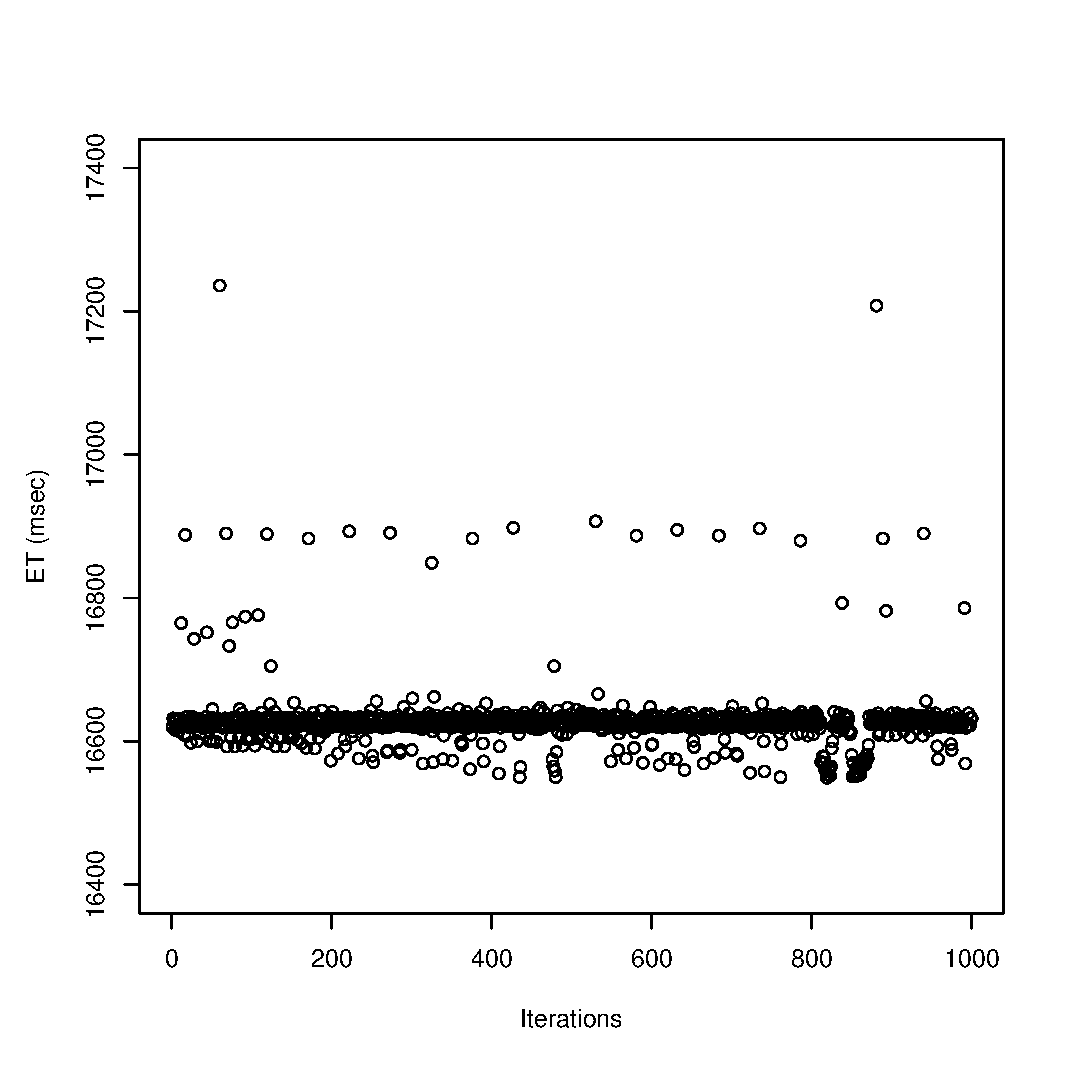
\includegraphics[scale=0.43]{figures/sodb8-ntp-on-turbo-on/16_sec_et_all.eps}
		\label{fig:16_sec_ect}
	}
	\subfigure[Per-execution ET on PUT32]{
		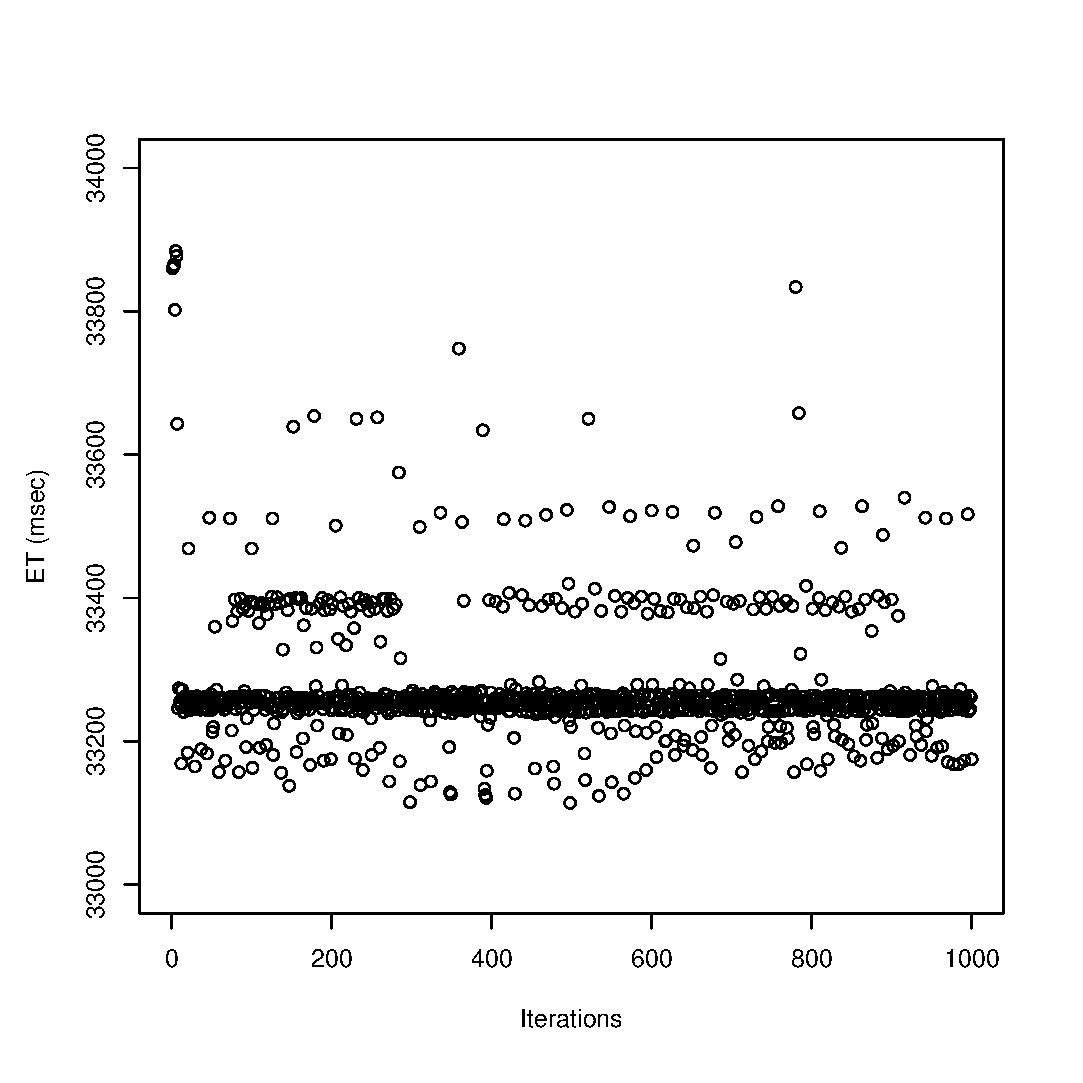
\includegraphics[scale=0.43]{figures/sodb8-ntp-on-turbo-on/32_sec_et_all.eps}
		\label{fig:32_sec_ect}
	}
	\caption{Per-execution ET on PUT16 and PUT32~\label{fig:et_plot}}
\end{figure}

\paragraph{Analysis} As illustrated in Figure~\ref{fig:16_sec_ect}, 
there was the compact band formed around 16,650 msecs in the $y$-axis corresponding to most of the PUT executions. 
Another {\it weak} band around 16,900 msecs was formed as well. 
Furthermore, Figure~\ref{fig:32_sec_ect} demonstrates this similar occurrence observed in PUT32. 
Most of the $y$-axis values were clustered around 33,250 msecs. 
There were also other higher bands consisting of around 33,400 or 33,500 msecs. 
For each experiment we indeed were able to see an intensively-clustered band (formed by around the median ET measurements) 
and a few bands weakly formed above and below the main band. 
%In particular, Y-axis values belonging to a higher band than the main band seem periodic. 

\paragraph{Hypothesis} ``{\it A high band seems formed 
due to daemon processes that periodically came up and ran for a moment, thus affecting 
ET at certain executions.}''

\paragraph{Test} 
When we looked at the data in PUT32, a raw ET value ({\it e.g}, 33,500 msecs) 
exceeding its median appeared at the 547th, 573th, 600th, and 626th. 
The same ET value was seen at the 731th, 758th, 916th, 942th, 968th, and 
995th. 
In other words, every 26 or 27 executions ET was higher than the median.
In PUT16, the measured high ET value was also observed every 51 executions. 
Based on these investigations, 
relatively more executed processes were included in the high ET measurements. 
Considering there were no other processes except PUT, 
we infer that some daemon processes must have contributed to forming such a high band. 
This hypothesis, therefore, is supported. 

\paragraph{Status} This cause is understood. 

\clearpage
\newpage

\subsection{Periodic Dips in PT}\label{sec:pd_pt}

We now turn our discussion to several phenomena regarding PT. 
PT is calculated as the sum of the user time and system time of PUT. 

\paragraph{Presumption} PT is totally flat. 

\paragraph{Description} 
In the measured data by EMPv2, 
we observed periodically-appearing dips. 
Figure~\ref{fig:pt_all} exhibits the distribution of PT in the experiments 
where the assigned task lengths were one, two, and four seconds. 

\begin{figure}[H]
	\centering
	\subfigure[Per-execution PT on PUT1]{
		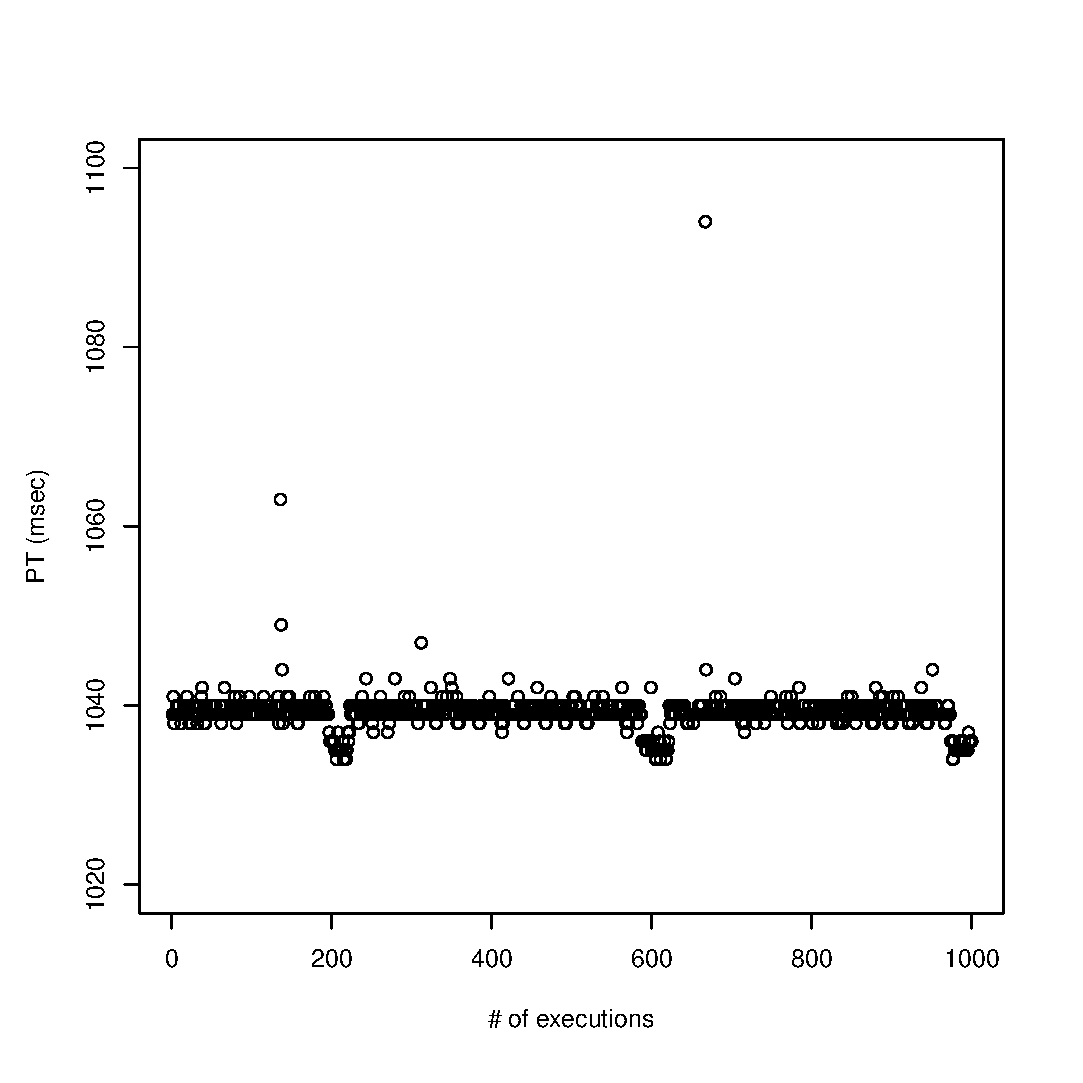
\includegraphics[scale=0.43]{figures/sodb8-ntp-on-turbo-on/1_sec_pt_all.eps}
		\label{fig:1_sec_pt_all}
	}
	\subfigure[Per-execution PT on PUT2]{
		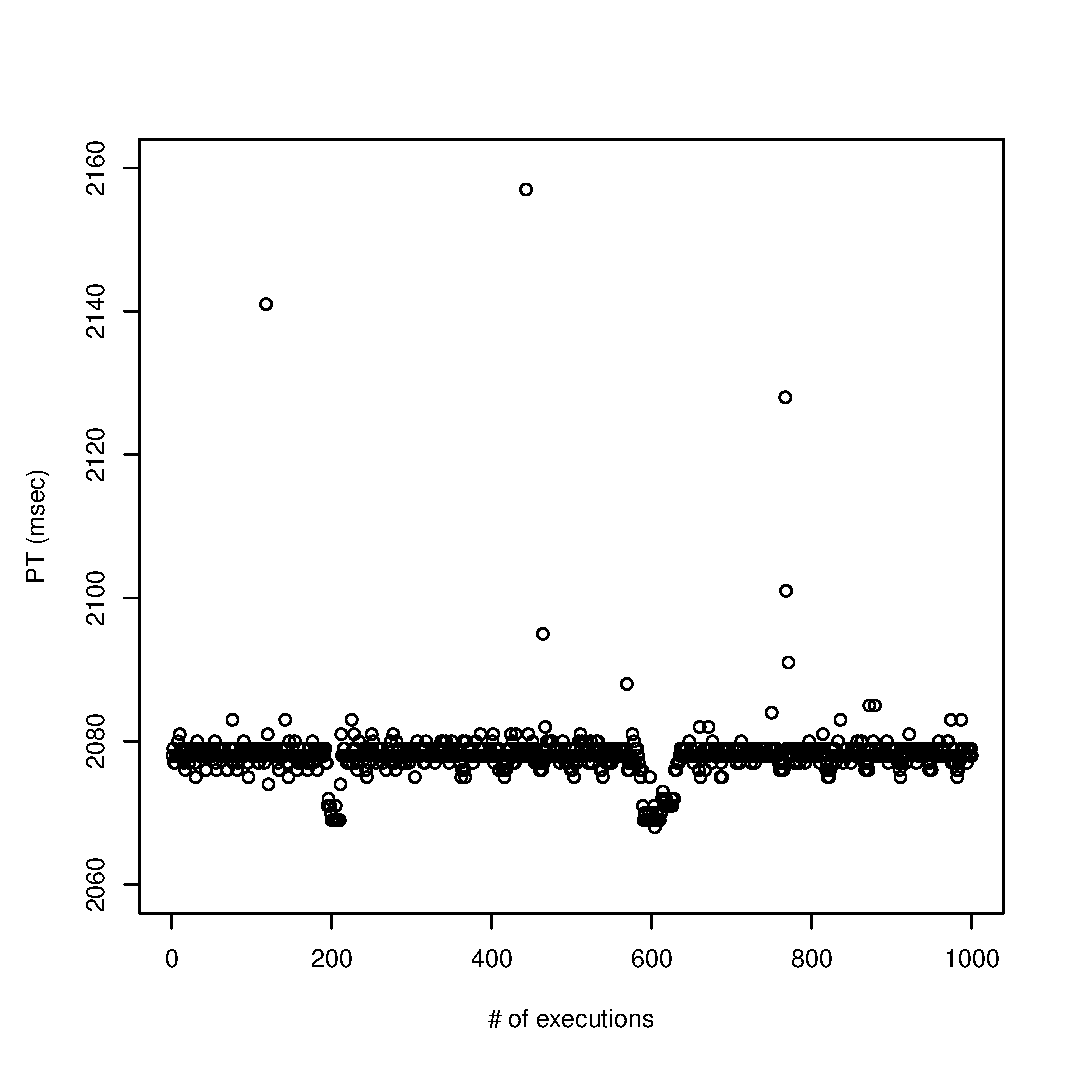
\includegraphics[scale=0.43]{figures/sodb8-ntp-on-turbo-on/2_sec_pt_all.eps}
		\label{fig:2_sec_pt_all}
	}
	\subfigure[Per-execution PT on PUT4]{
		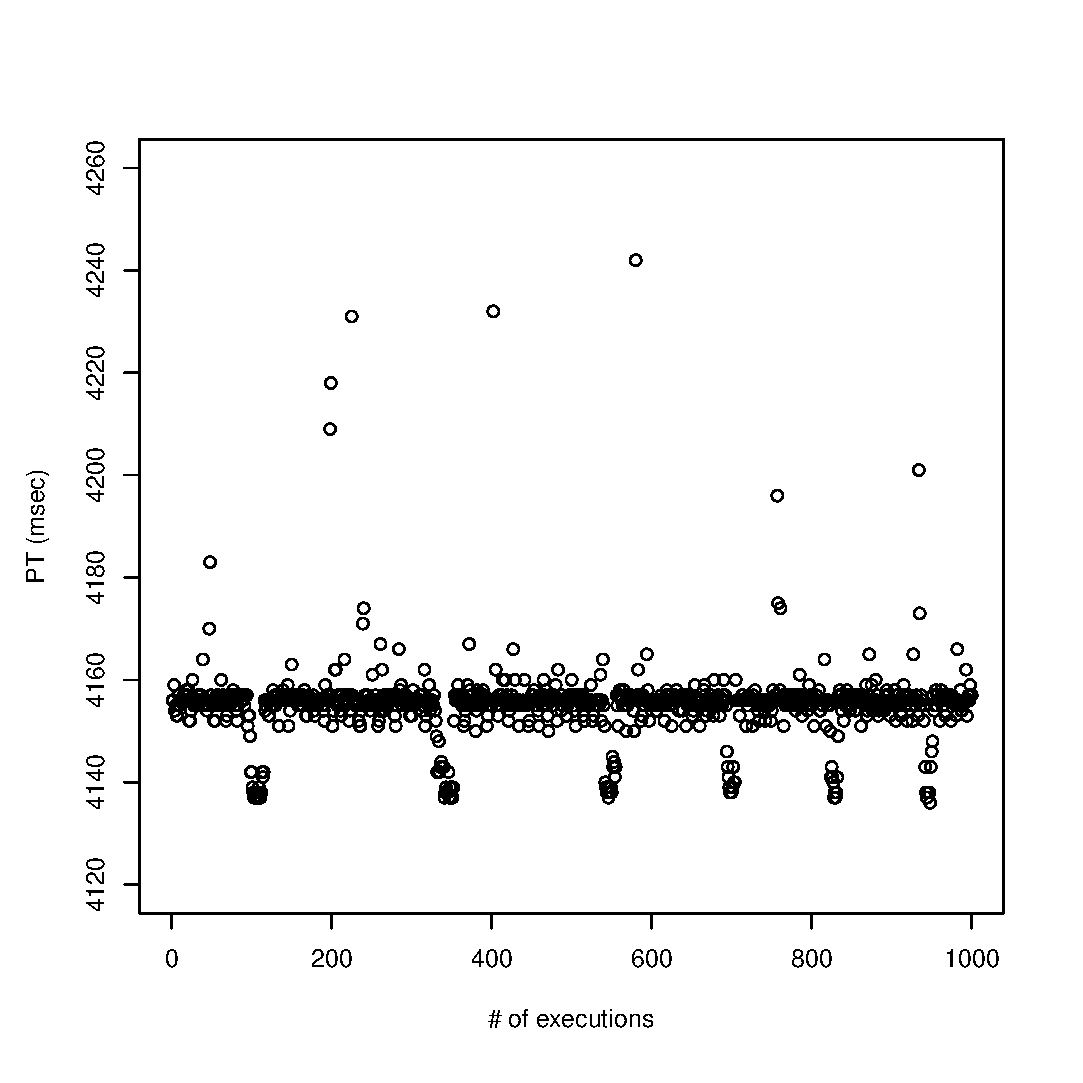
\includegraphics[scale=0.43]{figures/sodb8-ntp-on-turbo-on/4_sec_pt_all.eps}
		\label{fig:4_sec_pt_all}
	}
	\caption{Per-execution PT on PUT1, PUT2, and PUT4~\label{fig:pt_all}}
\end{figure}

\paragraph{Analysis}
At first, the calculated PT values were plotted around the median. 
At some point, however, the PT values dropped to the minimum, 
and then the values bounced back up to the median. 
This pattern repeated after a certain number of executions; 
namely, this dip seemed to occur every around $x$ seconds after the first appearance. 
Specifically, the dip first appeared after the 200th execution (about 200 seconds) and 
reappeared every approximately 400 seconds, as shown in Figure~\ref{fig:1_sec_pt_all}.
In PUT2, these dips first emerged around the 200th execution, 
and they reoccurred after around 800 seconds, as illustrated in Figure~\ref{fig:2_sec_pt_all}.
In Figure~\ref{fig:4_sec_pt_all}, 
the first dip was observed at around the 100th execution and repeated after approximately 800 seconds. 
Note that the $x$-axis values represents execution number, rather than actual time.
The same execution number across different tasks do not mean that the respective actual times are same. 
The 200th execution in PUT2 and PUT4 could happen around 400 seconds and 800 seconds, respectively, after the tasks start.
%Although weak, the dips seem to occur every around 400 seconds even in the eight-second task. 

\paragraph{Hypothesis I} ``{\it These dips are caused by adjustments by NTP (Network Time Protocol)~\cite{Mills} used to 
synchronize its local system time to a server in the network.}''

This hypothesis is based on the assumption that PT will be faster whenever the system time is corrected 
by the NTP daemon ({\tt ntpd}). 

\paragraph{Test} To confirm this, we ran some additional experiments in which {\tt ntpd} was disabled.
In these experiments, EMPv1 was used. 

The experiment results are shown in Figure~\ref{fig:ntpd_off_pt}. 
Unfortunately, the dips did not go away. 
Conversely, overall dips became thinner and appeared more frequently. 
For instance, the dips shown in Figure~\ref{fig:ntp_off_1_sec_pt_all} were weaker and more frequent, 
compared with the ones in Figure~\ref{fig:1_sec_pt_all}. 
The same trend was seen in Figures~\ref{fig:ntp_off_2_sec_pt_all} and~\ref{fig:ntp_off_4_sec_pt_all} although less strong and somewhat seemingly random. 
In addition, the overall distribution of PT looked more dispersed, weakening the compactness of the bands.

\begin{figure}[H]
	\centering
	\subfigure[Per-execution PT on PUT1]{
		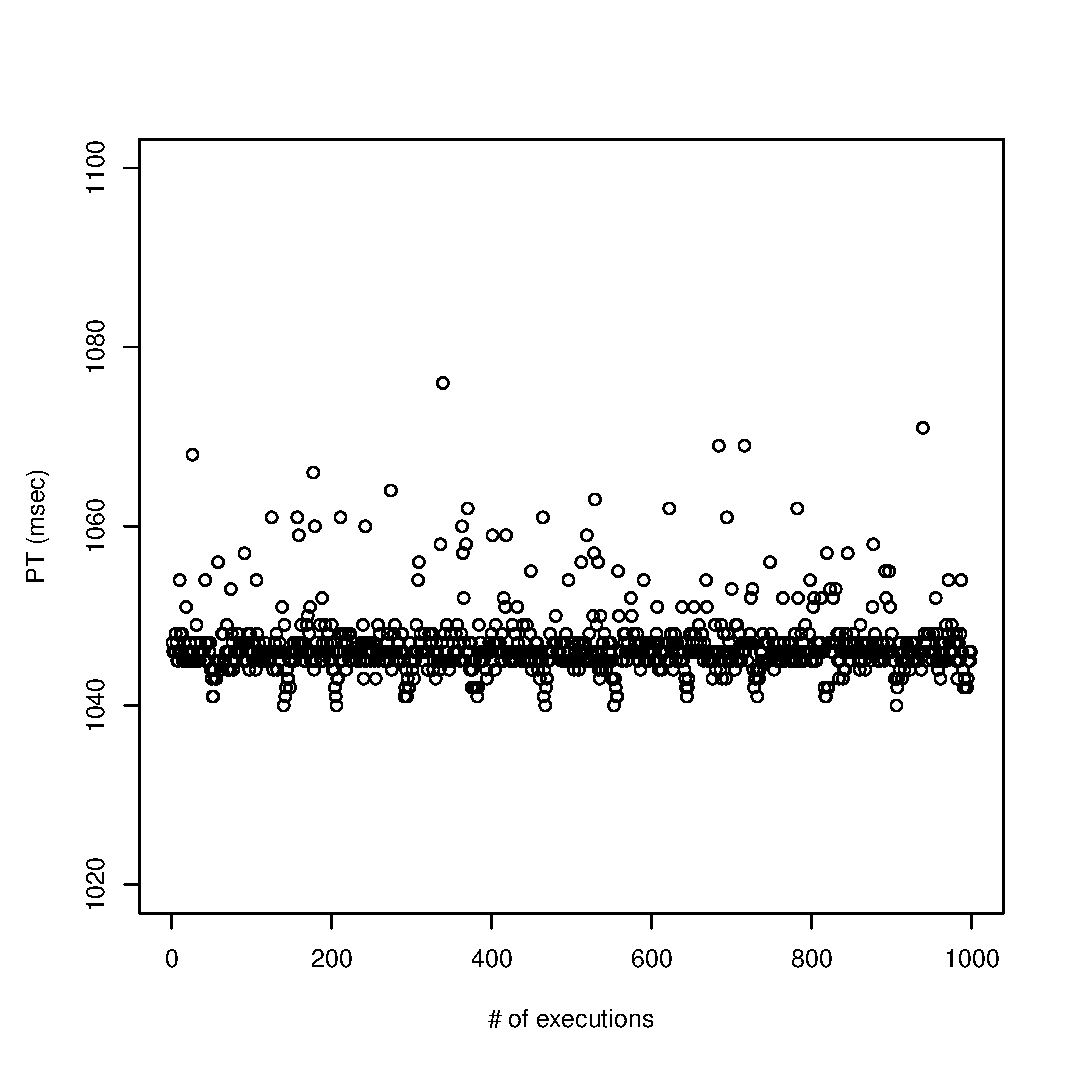
\includegraphics[scale=0.43]{figures/sodb8-ntp-off-turbo-on/1_sec_pt_all.eps}
		\label{fig:ntp_off_1_sec_pt_all}
	}
	\subfigure[Per-execution PT on PUT2]{
		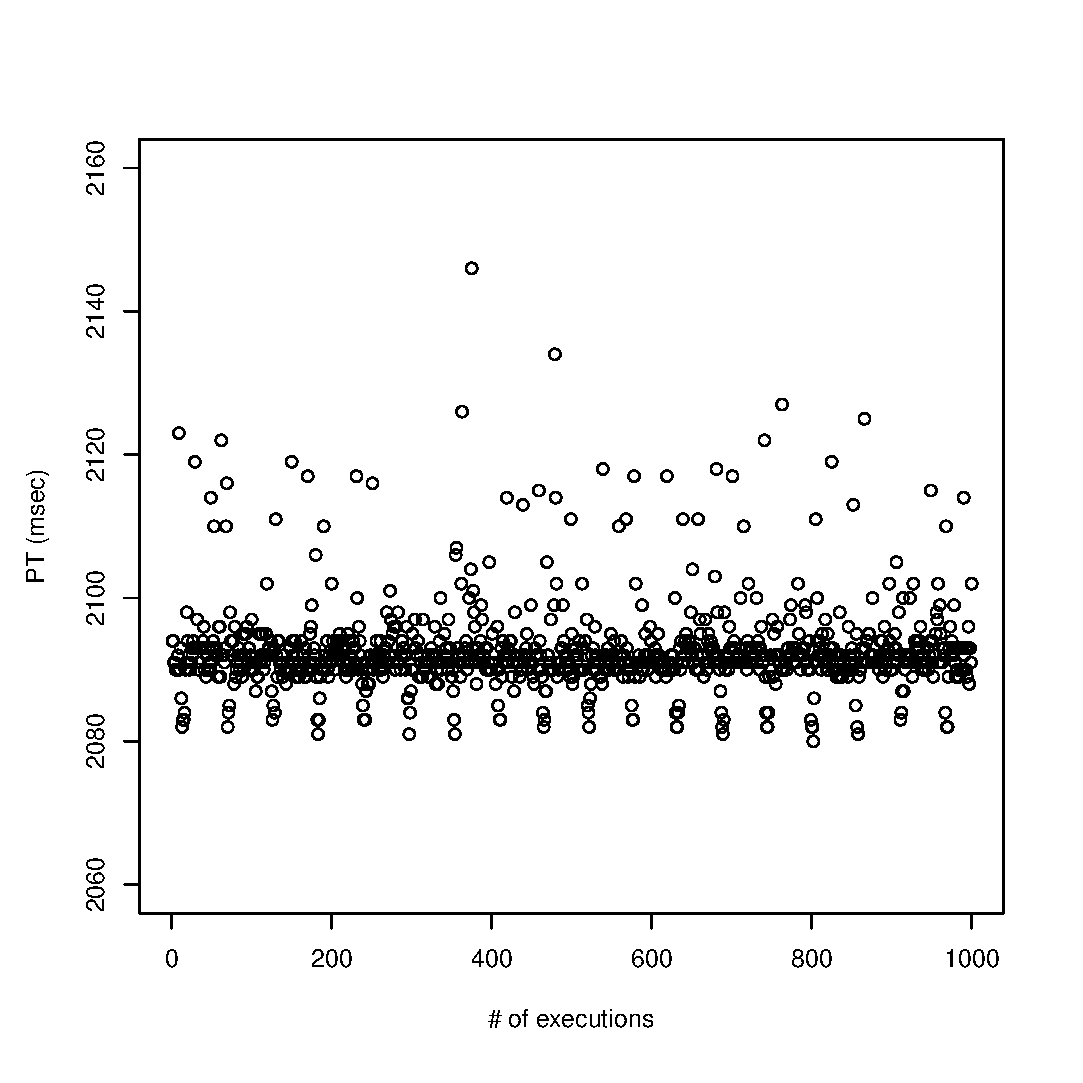
\includegraphics[scale=0.43]{figures/sodb8-ntp-off-turbo-on/2_sec_pt_all.eps}
		\label{fig:ntp_off_2_sec_pt_all}
	}
	\subfigure[Per-execution PT on PUT4]{
		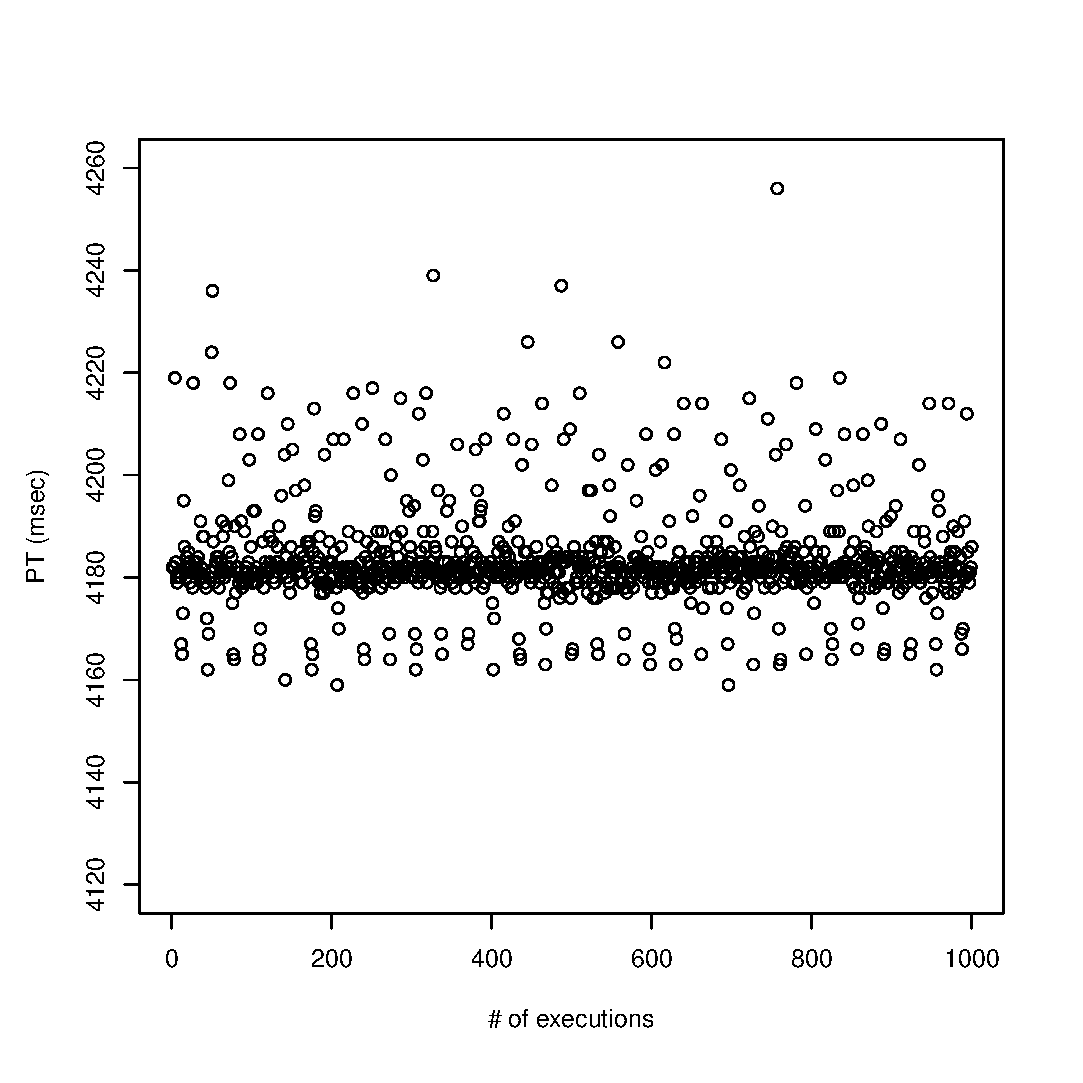
\includegraphics[scale=0.43]{figures/sodb8-ntp-off-turbo-on/4_sec_pt_all.eps}
		\label{fig:ntp_off_4_sec_pt_all}
	}
	\caption{Per-execution PT on PUT1, PUT2, and PUT4 when {\tt ntpd} was turned off~\label{fig:ntpd_off_pt}}
\end{figure}

Turning off {\tt ntpd} did not help us to figure out the cause of the dips. 
Our hypothesis, thus, is not supported.

\paragraph{Hypothesis II} ``{\it Disabling the Turbo mode set in a processor will make the dips go away.}''

Some processors support ``turbo mode'' and scale up the frequency and voltage at times. 
This hypothesis studies the impact of the frequency scaling caused by the turbo mode. 

%Turbo mode dynamically increases the processor's frequency as needed by taking advantage of thermal and power headroom. 
%Speedstep is meant to reduce power usage/heat based on the load of the processor. (slow down an idle processor)
%Turbo boost increase processor speed based on load and temperature. So it will find the so called sweet spot between temperature and performance up to a certain clock speed.

\paragraph{Test} 
We found that the processor type of our experiment machine is Intel Core {\it i}7 CPU 870 @ 2.93GHz. 
This processor enabled by default the turbo mode through the feature named ``Intel$\textregistered$ Turbo Boost Technology''. 
In addition, the turbo mode can be influenced by another feature of the processor, 
called ``Enhanced Intel SpeedStep$\textregistered$ Technology'', which can reduce power usage/heat based on the load of the processor. 
To see if the Turbo mode was the cause of the dips, we disabled both features. The frequency scaling was stopped.

Figure~\ref{fig:turbo_off_pt} shows the distribution of PT on PUT1, PUT2, and PUT4. 
In these data, EMPv2 was used. 
Compared with Figure~\ref{fig:pt_all}, overall the degree of dips became much more discrete and weaker. 
In addition, the standard variations of PT on the PUT tasks reduced to 
1.65/2.78/5.75 from 2.39/4.33/7.52, respectively. 
This implies that turning off the turbo mode helped us reduce the variation of PT. 
As a result, most executions yielded flat PT measurements.
Nevertheless, the dips were still observed.

\begin{figure}[H]
	\centering
	\subfigure[Per-execution PT on PUT1]{
		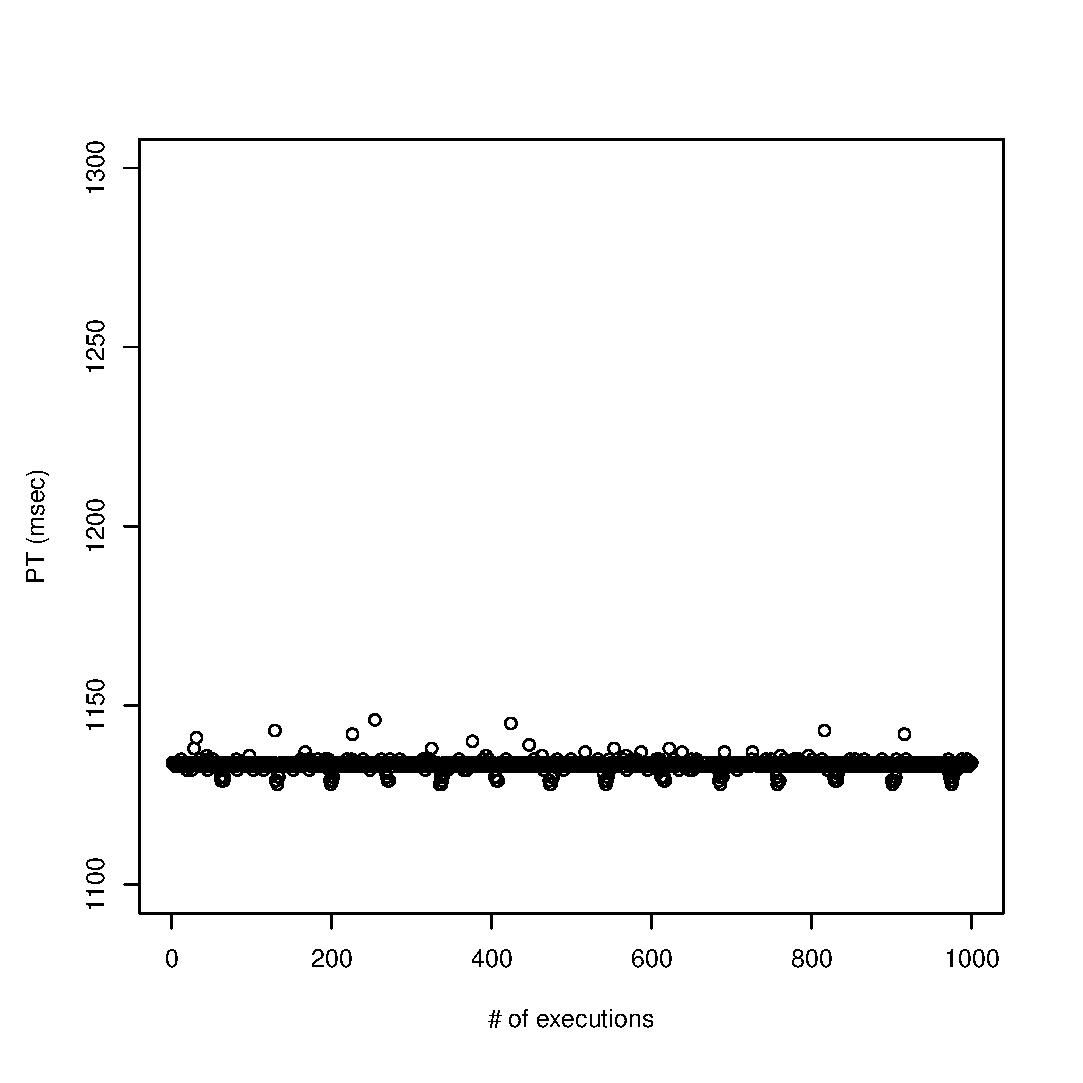
\includegraphics[scale=0.43]{figures/sodb8-ntp-on-turbo-off/1_sec_pt_all.eps}
		\label{fig:tm_1_sec_pt_all}
	}
	\subfigure[Per-execution PT on PUT2]{
		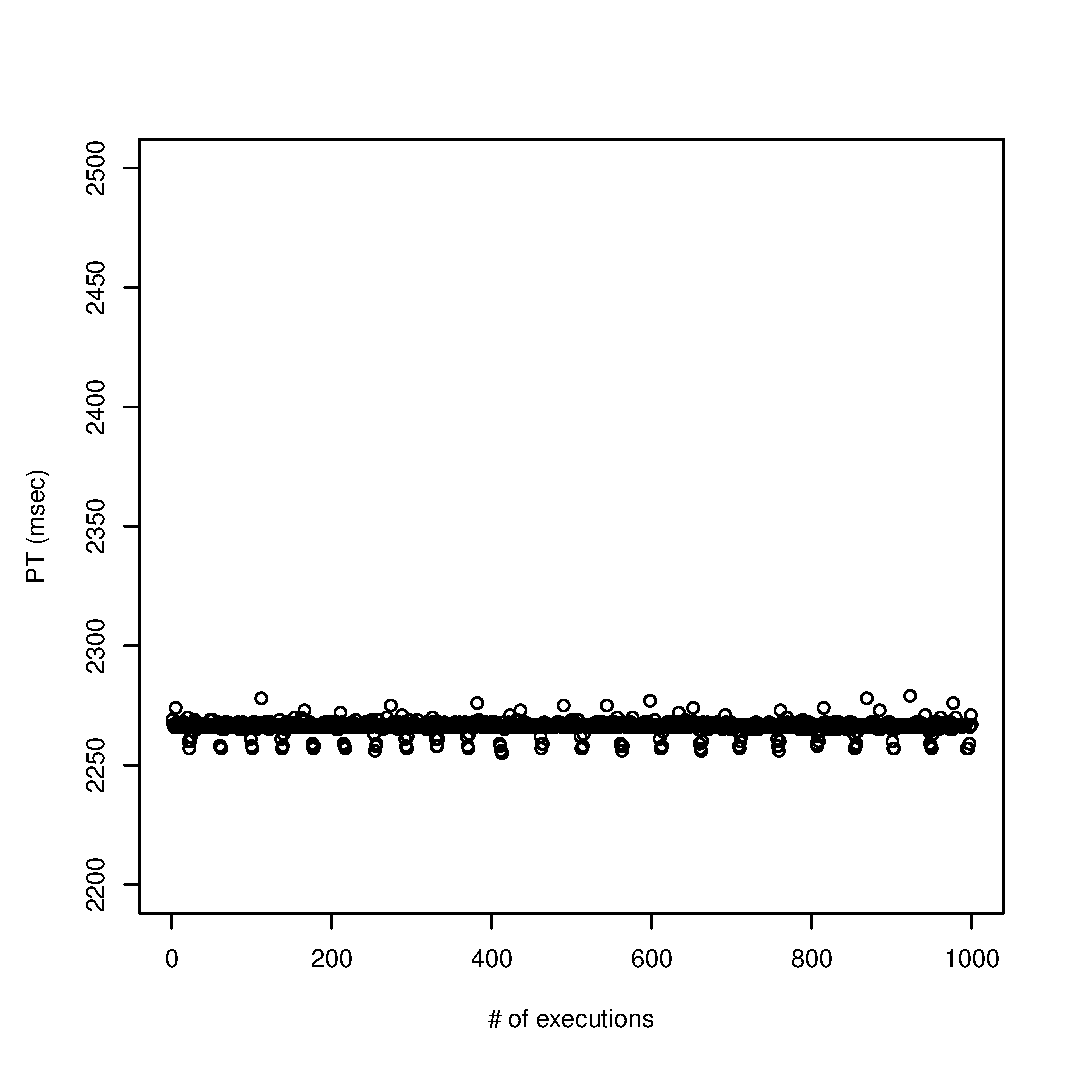
\includegraphics[scale=0.43]{figures/sodb8-ntp-on-turbo-off/2_sec_pt_all.eps}
		\label{fig:tm_2_sec_pt_all}
	}
	\subfigure[Per-execution PT on PUT4]{
		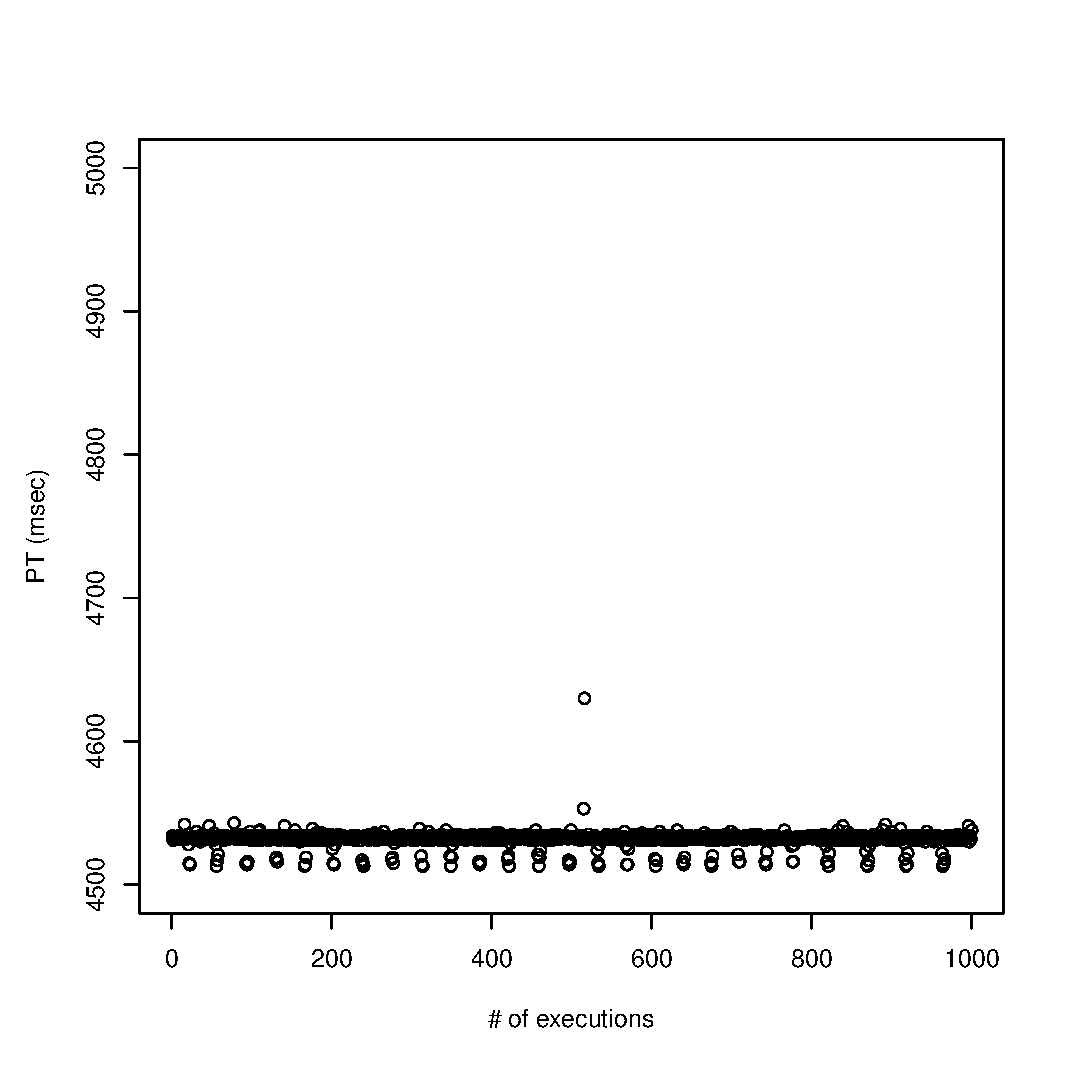
\includegraphics[scale=0.43]{figures/sodb8-ntp-on-turbo-off/4_sec_pt_all.eps}
		\label{fig:tm_4_sec_pt_all}
	}
	\caption{Per-execution PT on PUT1, PUT2, PUT4, and PUT8 when the turbo mode was turned off~\label{fig:turbo_off_pt}}
\end{figure}

%As shown in Figures~\ref{fig:turbo_off_pt}, overall PT was flat although the dots look scattered due to resolution . 
%Specifically, the standard variations of PT in the 1/2/4-second tasks reduced to 1.65/2.78/5.75 from 2.39/4.33/7.52, respectively. 

%Figure~\ref{fig:turbo_off_ect} shows the distribution of ET in the one-/two-/four-second tasks. 
%Interestingly, the 
%
%\begin{figure}[htp!]
%	\centering
%	\subfigure[Per-execution ET on the 1-second task]{
%		\includegraphics[scale=0.43]{figures/turbo_mode/1_sec_ect_all.eps}
%		\label{fig:tm_1_sec_ect_all}
%	}
%	\subfigure[Per-execution ET on the 2-second task]{
%		\includegraphics[scale=0.43]{figures/turbo_mode/2_sec_ect_all.eps}
%		\label{fig:tm_2_sec_ect_all}
%	}
%	\subfigure[Per-execution ET on the 4-second task]{
%		\includegraphics[scale=0.43]{figures/turbo_mode/4_sec_ect_all.eps}
%		\label{fig:tm_4_sec_ect_all}
%	}
%%	\subfigure[Per-execution PT on the 8-second task]{
%%		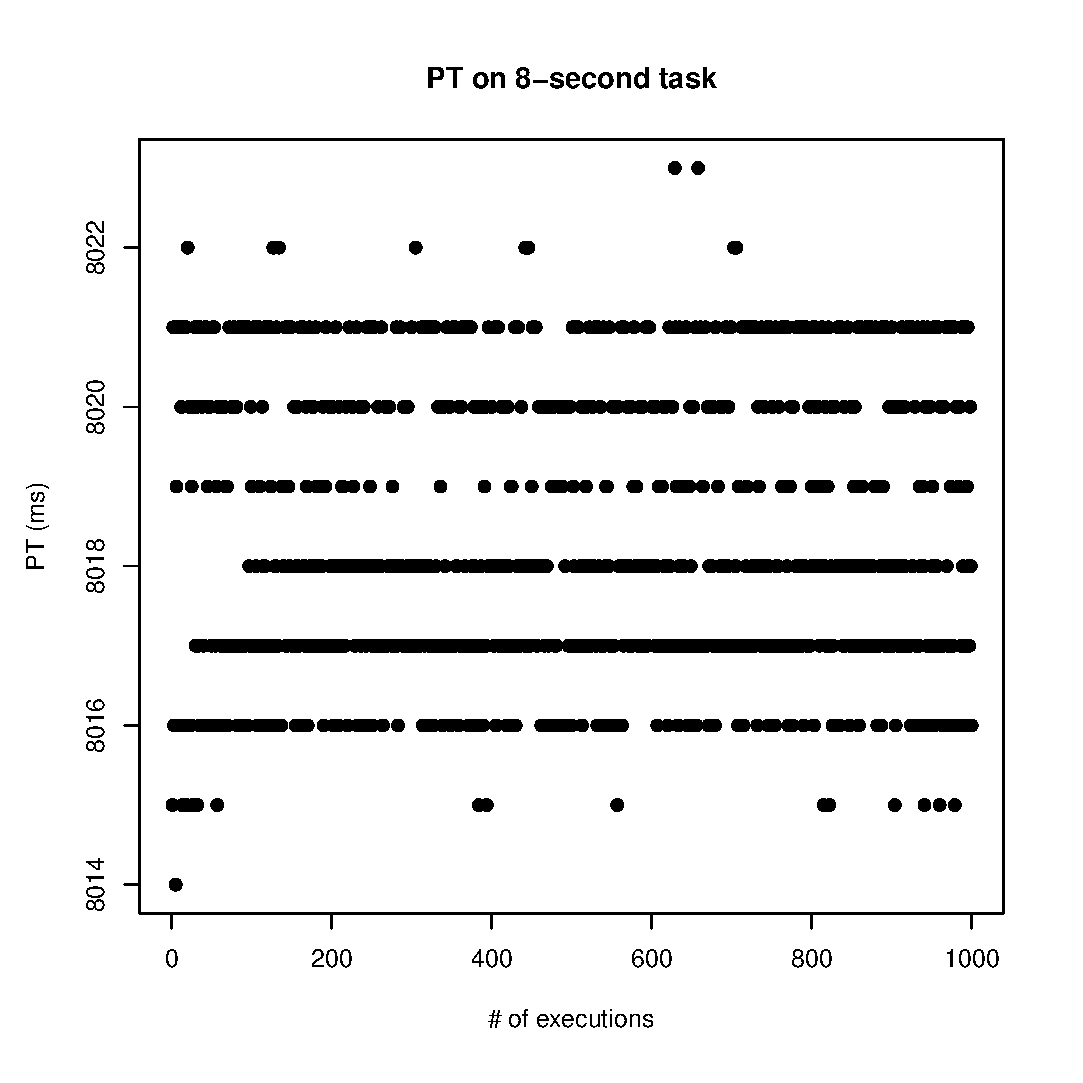
\includegraphics[scale=0.43]{figures/ntp-off/8_sec_pt_all.eps}
%%		\label{fig:ntp_off_8_sec_pt_all}
%%	}
%%	\caption{Per-execution PT on the 1/2/4/8-second task when {\tt ntpd} was turned off\label{fig:ntpd_off_pt}}
%	\caption{Per-execution ET on the 1/2/4-second task when Turbo mode was turned off\label{fig:turbo_off_ect}}
%\end{figure}
%
%They all look flat except a couple of executions.

\paragraph{Status} This cause is yet understood. 

In subsequent sections, we show the experiment results after the Turbo mode was off.

\newpage

\subsection{Synchronized ET and PT}

\paragraph{Presumption} Totally correlated

\paragraph{Description} 
Figure~\ref{fig:sync_time} shows ET and PT measurements on PUT2 and PUT4. 
The common phenomenon is that most of the measured ET and PT data looked synchronized. 
The phenomenon was observed from the EMPv3 data. 

\begin{figure}[H]
	\centering
	\subfigure[Per-execution ET on PUT2]{
		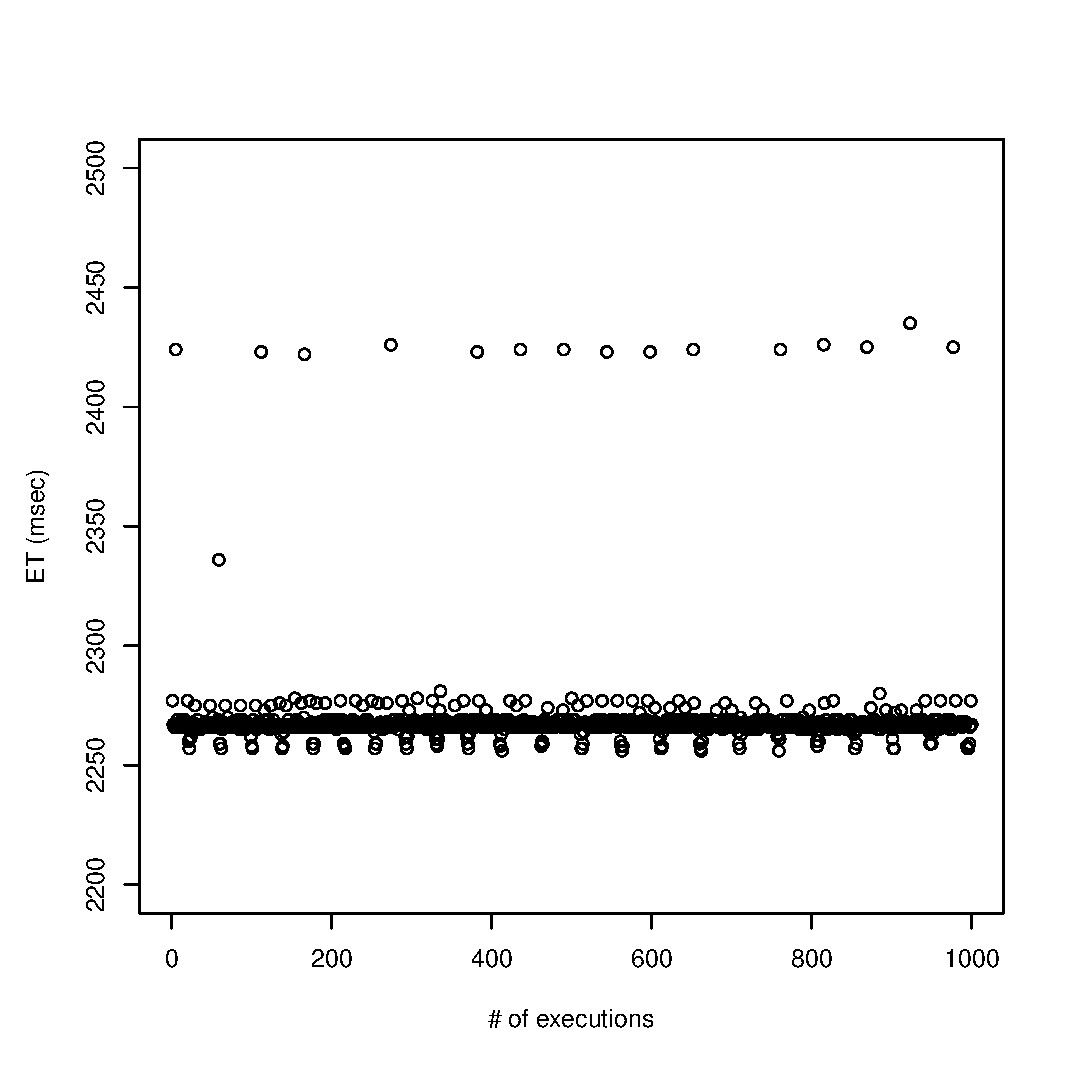
\includegraphics[scale=0.43]{figures/sodb8-ntp-on-turbo-off/2_sec_et_all.eps}
		\label{fig:2_sec_ect}
	}
	\subfigure[Per-execution PT on PUT2]{
		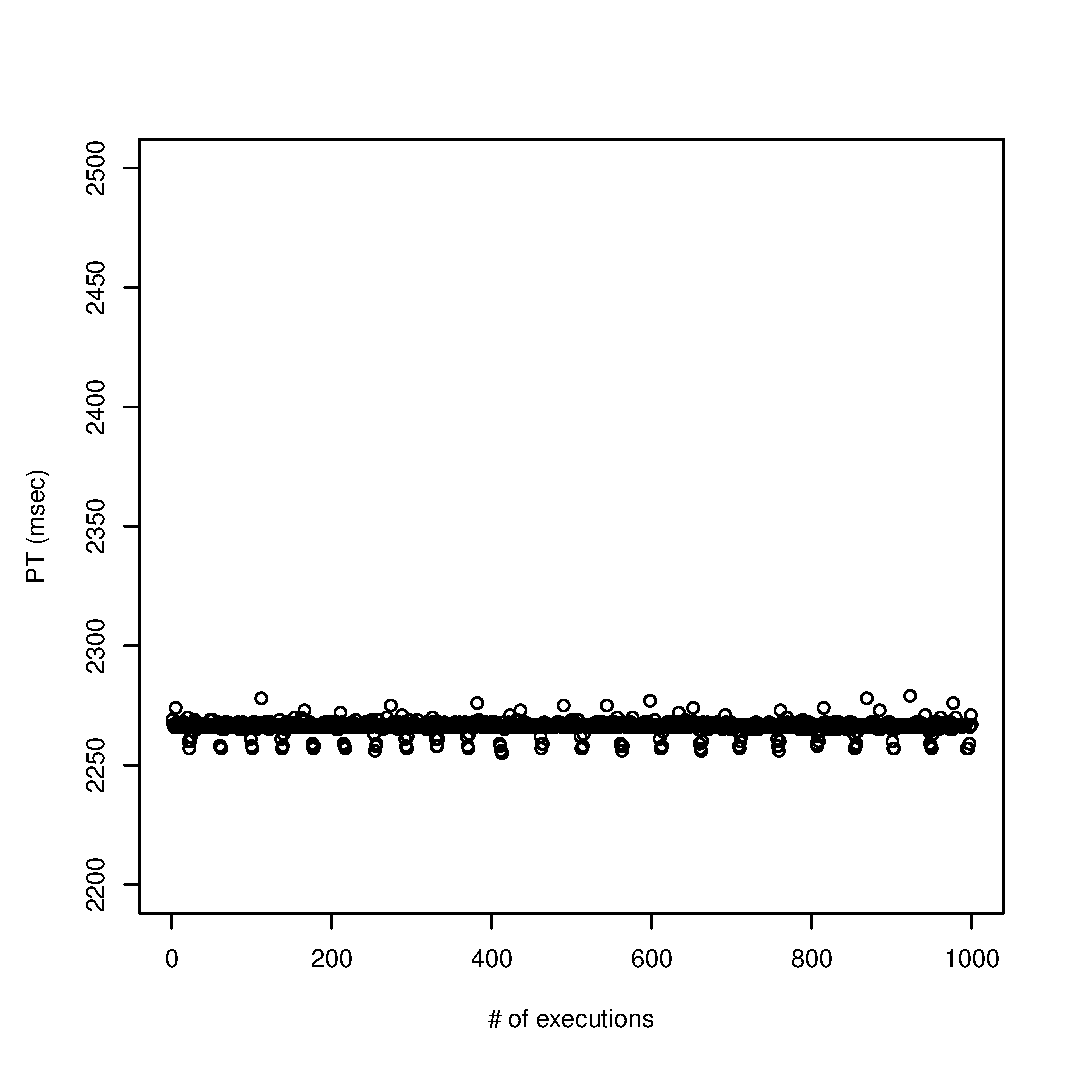
\includegraphics[scale=0.43]{figures/sodb8-ntp-on-turbo-off/2_sec_pt_all.eps}
		\label{fig:2_sec_pt_all2}
	}
	\subfigure[Per-execution ET on PUT4]{
		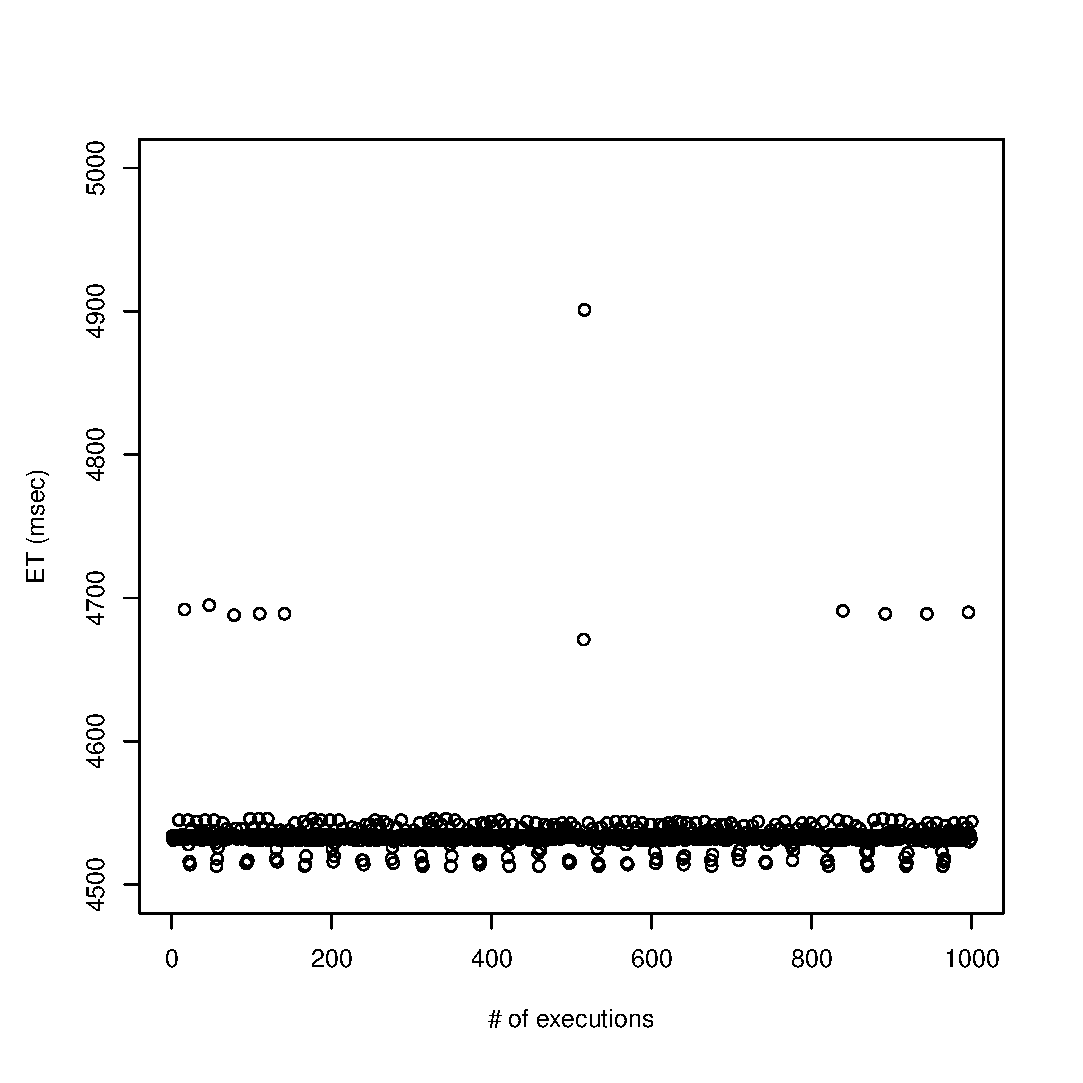
\includegraphics[scale=0.43]{figures/sodb8-ntp-on-turbo-off/4_sec_et_all.eps}
		\label{fig:4_sec_ect}
	}
	\subfigure[Per-execution PT on PUT4]{
		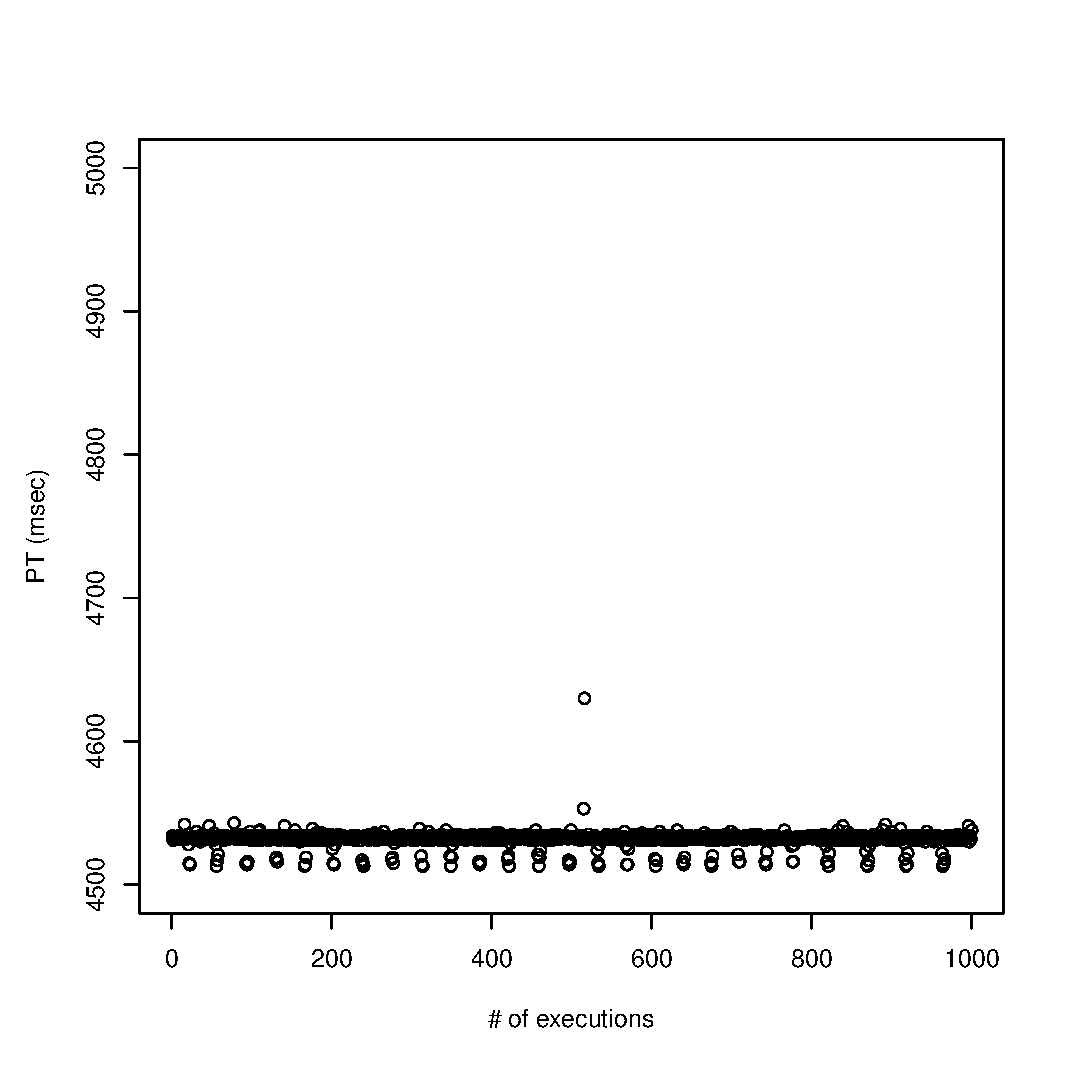
\includegraphics[scale=0.43]{figures/sodb8-ntp-on-turbo-off/4_sec_pt_all.eps}
		\label{fig:4_sec_pt_all2}
	}
	\caption{Per-execution ET/PT on PUT2 and PUT4~\label{fig:sync_time}}
\end{figure}

\paragraph{Analysis} In PUT2, if we overlap Figures~\ref{fig:2_sec_ect} and \ref{fig:2_sec_pt_all2}, 
we know that most executions have exactly the same ET and PT. 
This also holds true for PUT4, as shown in Figures~\ref{fig:4_sec_ect} and \ref{fig:4_sec_pt_all2}. 
The synchronization does not take place in some executions, where some other daemon processes had indeed run together.

%\paragraph{Hypothesis} ``{\it When the number of daemon processes is very low, ET and PT will be synchronized.}''. 
%
%\paragraph{Test} 
%For this test, we used EMPv2. 
%Figure~\ref{fig:daemon} shows the number of daemon processes observed when measuring the execution time of PUT2 and PUT4.
%In Figures~\ref{fig:2_sec_low_daemon} and \ref{fig:4_sec_low_daemon}, 
%we found that when fewer than three daemon processes (low) was present, 
%ET and PT measurements were exactly the same. 
%Figures~\ref{fig:2_sec_high_daemon} and \ref{fig:4_sec_high_daemon} exhibit the measurements with 
%more than three daemon processes (high). 
%For these measurements, both did not get synchronized; 
%namely, the measured ET values were greater than the measured PT values. 
%This hypothesis, therefore, is supported. 
%
%\begin{figure}[hp!]
%	\centering
%	\subfigure[Low number of daemon processes]{
%		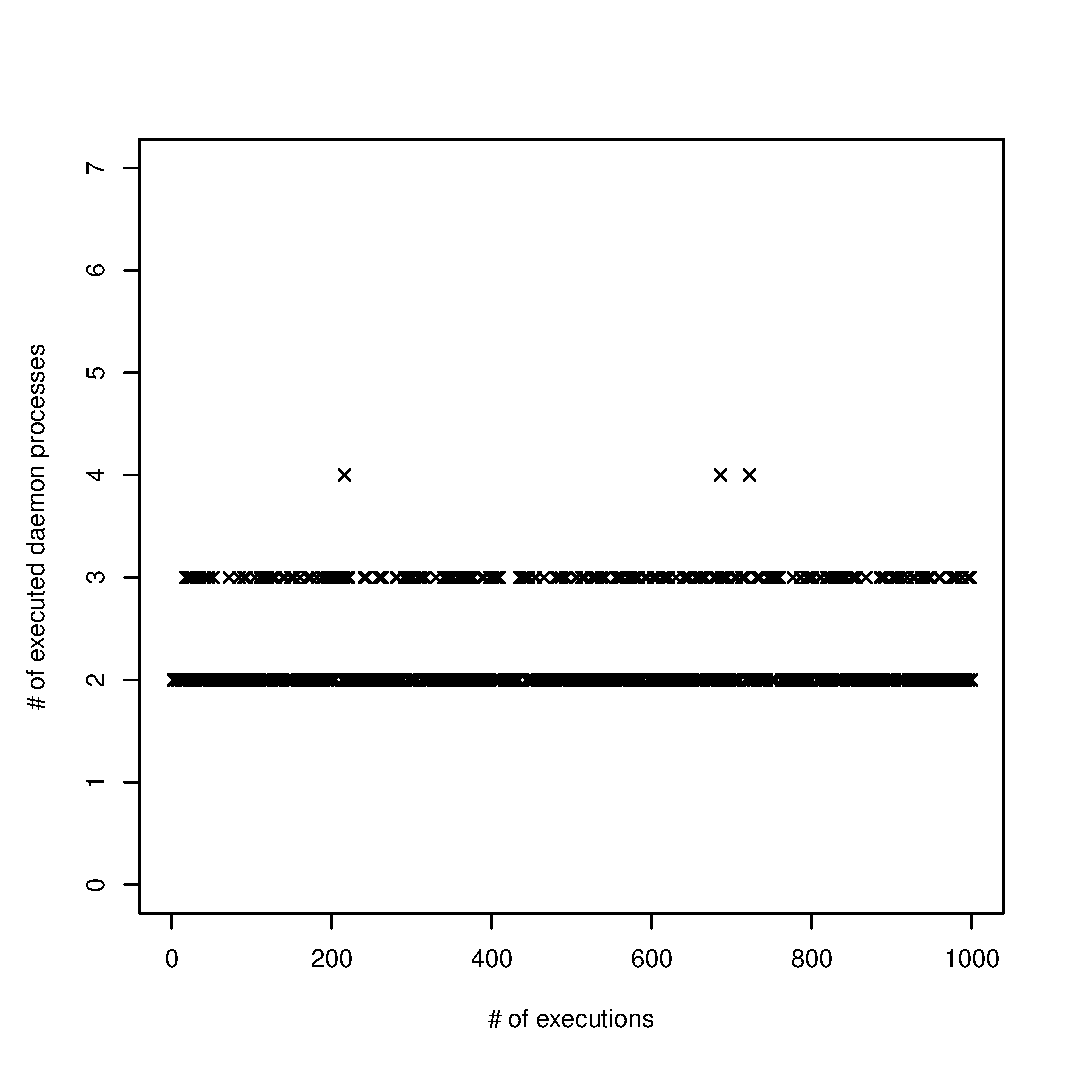
\includegraphics[scale=0.43]{figures/sodb8-ntp-on-turbo-on/2_sec_num_low_daemons.eps}
%		\label{fig:2_sec_low_daemon}
%	}
%	\subfigure[High number of daemon processes]{
%		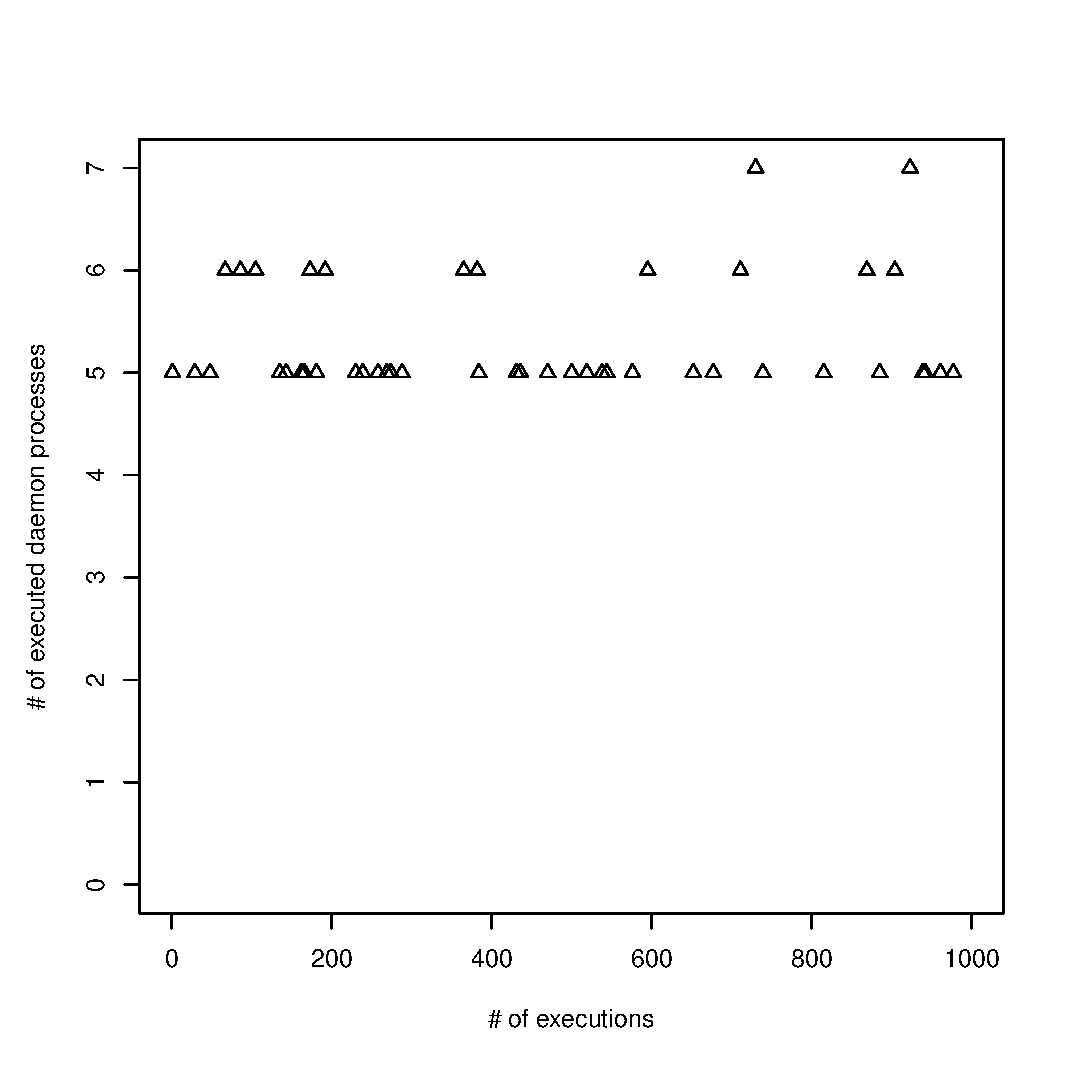
\includegraphics[scale=0.43]{figures/sodb8-ntp-on-turbo-on/2_sec_num_high_daemons.eps}
%		\label{fig:2_sec_high_daemon}
%	}
%	\subfigure[Low number of daemon processes]{
%		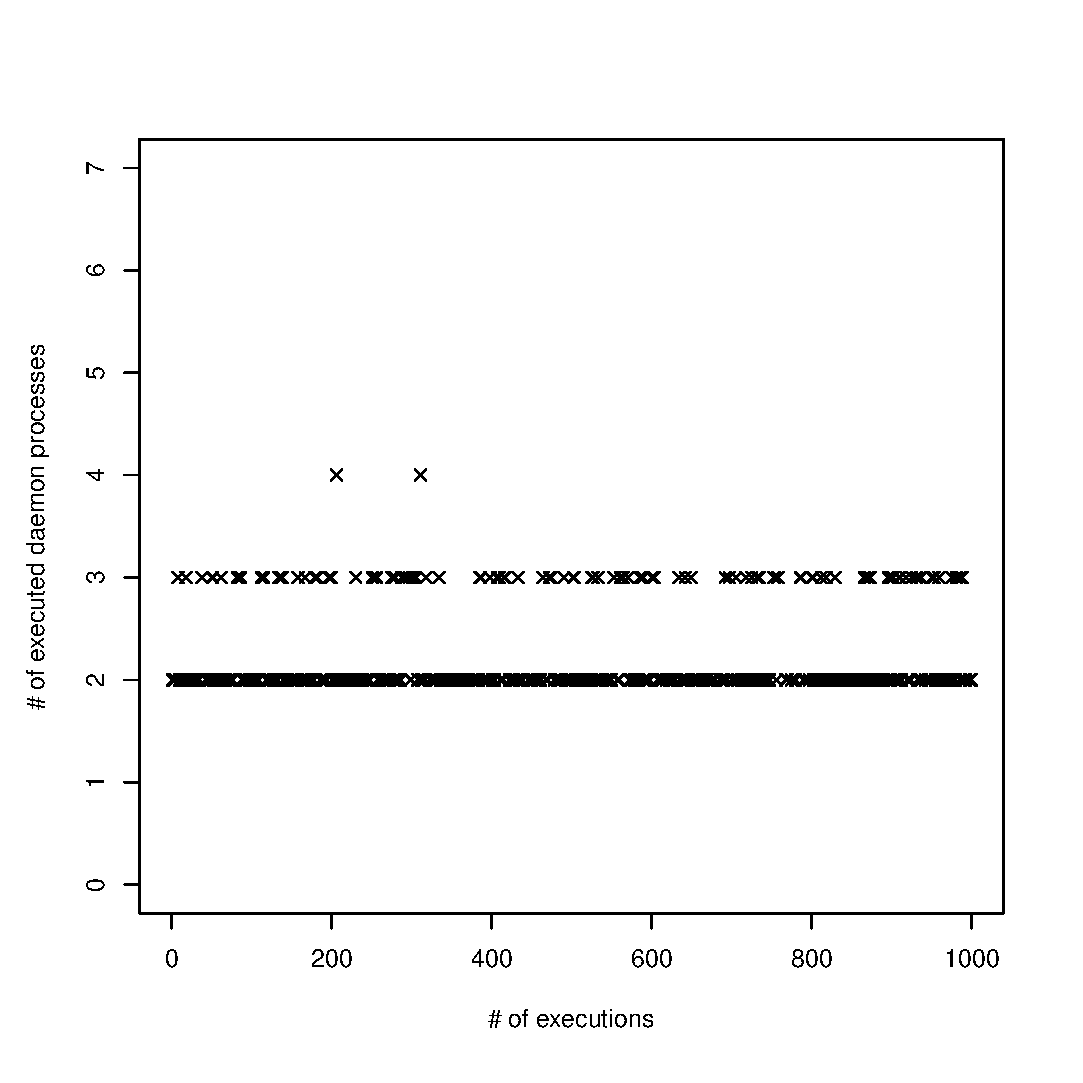
\includegraphics[scale=0.43]{figures/sodb8-ntp-on-turbo-on/4_sec_num_low_daemons.eps}
%		\label{fig:4_sec_low_daemon}
%	}
%	\subfigure[High number of daemon processes]{
%		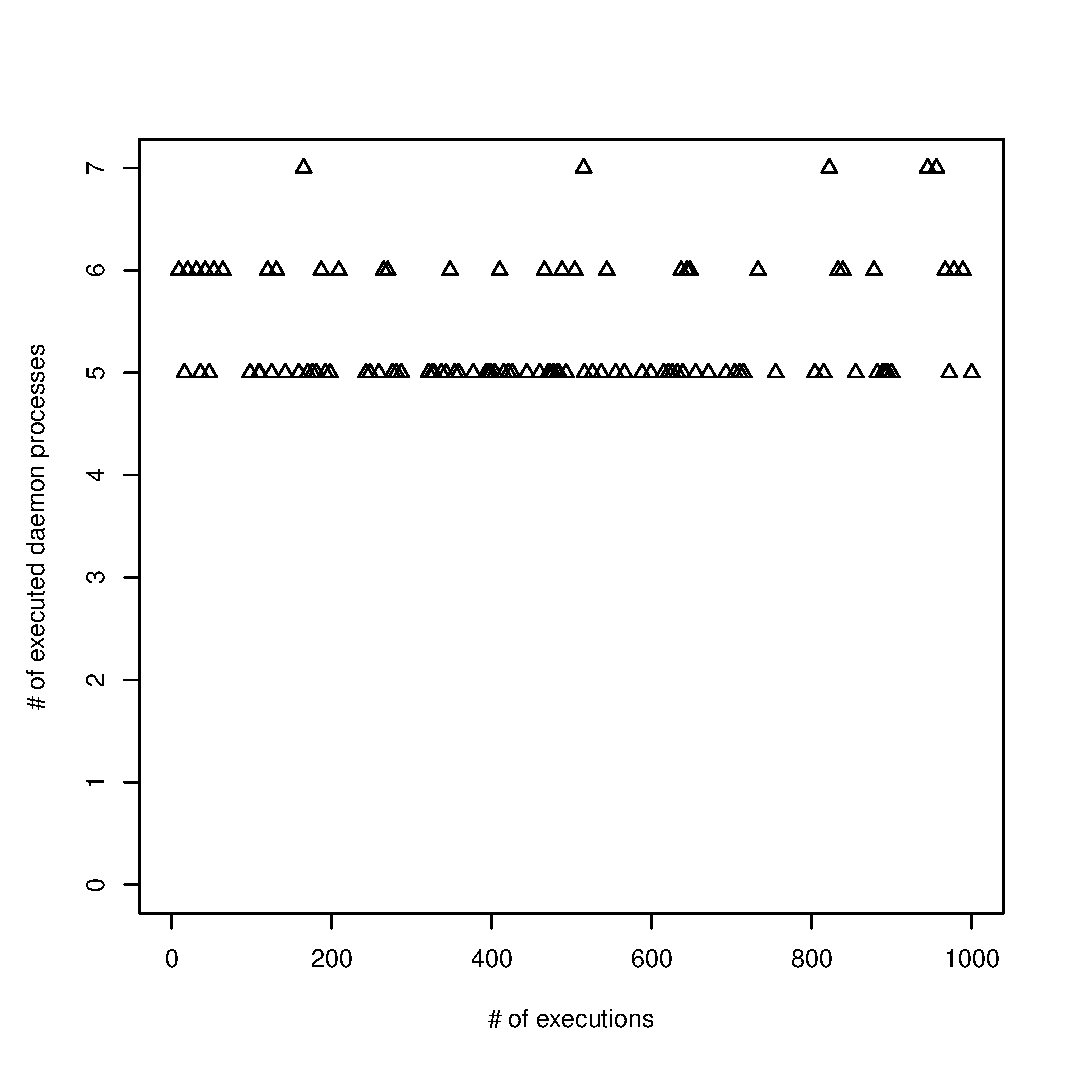
\includegraphics[scale=0.43]{figures/sodb8-ntp-on-turbo-on/4_sec_num_high_daemons.eps}
%		\label{fig:4_sec_high_daemon}
%	}
%	\caption{Number of daemon processes per execution\label{fig:daemon}}
%\end{figure}
%
%\paragraph{Status} We understood this.

\newpage

\subsection{Outliers in PT}

\paragraph{Presumption} Large outlier in PT should not occur. 

\paragraph{Description} 
This phenomenon indicates that a couple of PT measurements showed exceedingly high peaks. 

\paragraph{Analysis} 
%In Figure~\ref{fig:pt_all}, we've already seen several outliers across different measurements.
%There is one outlier observed on PUT8, as shown in Figure~\ref{fig:1_sec_pt_all}, 
%and there are also several outliers seen in Figures~\ref{fig:1_sec_pt_all} and \ref{fig:4_sec_pt_all}. 
%Furthermore, we can see these abnormal PT in heavier tasks. 

Figure~\ref{fig:peak_pt} exhibits the PT measurements on PUT16, PUT32, and PUT64. 
These data were obtained by EMPv3. 
There were three outliers observed at around the 90th and the 820th executions, as shown in Figure~\ref{fig:16_sec_pt_all}.
Likewise, a couple of outliers were also observed from the measurements on PUT32 and in PUT64, 
as illustrated in Figures~\ref{fig:32_sec_pt_all} and \ref{fig:64_sec_pt_all}.

\begin{figure}[H]
\centering
	\subfigure[Per-execution PT on PUT16]{
		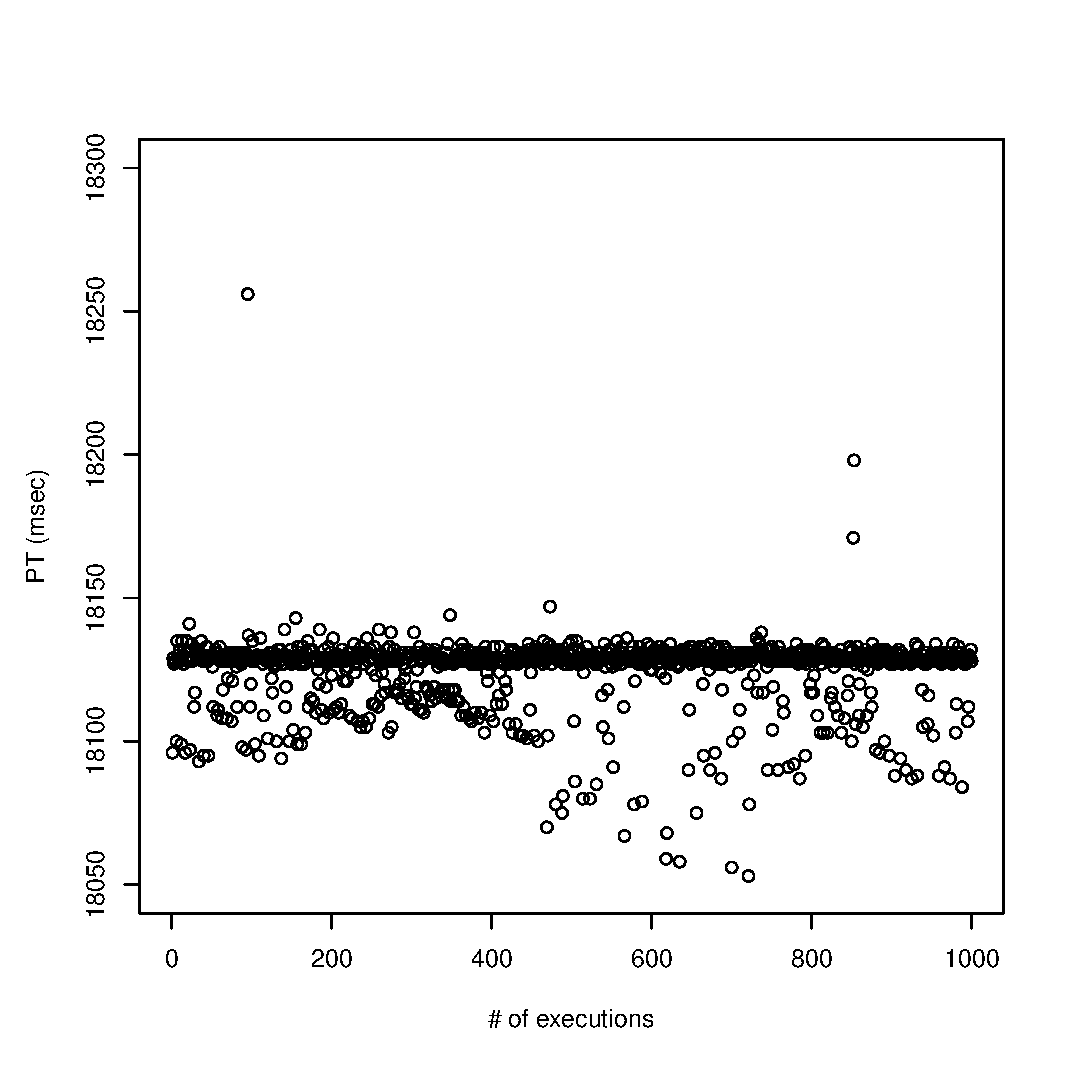
\includegraphics[scale=0.43]{figures/sodb8-ntp-on-turbo-off/16_sec_pt_all.eps}
		\label{fig:16_sec_pt_all}
	}
	\subfigure[Per-execution PT on PUT32]{
		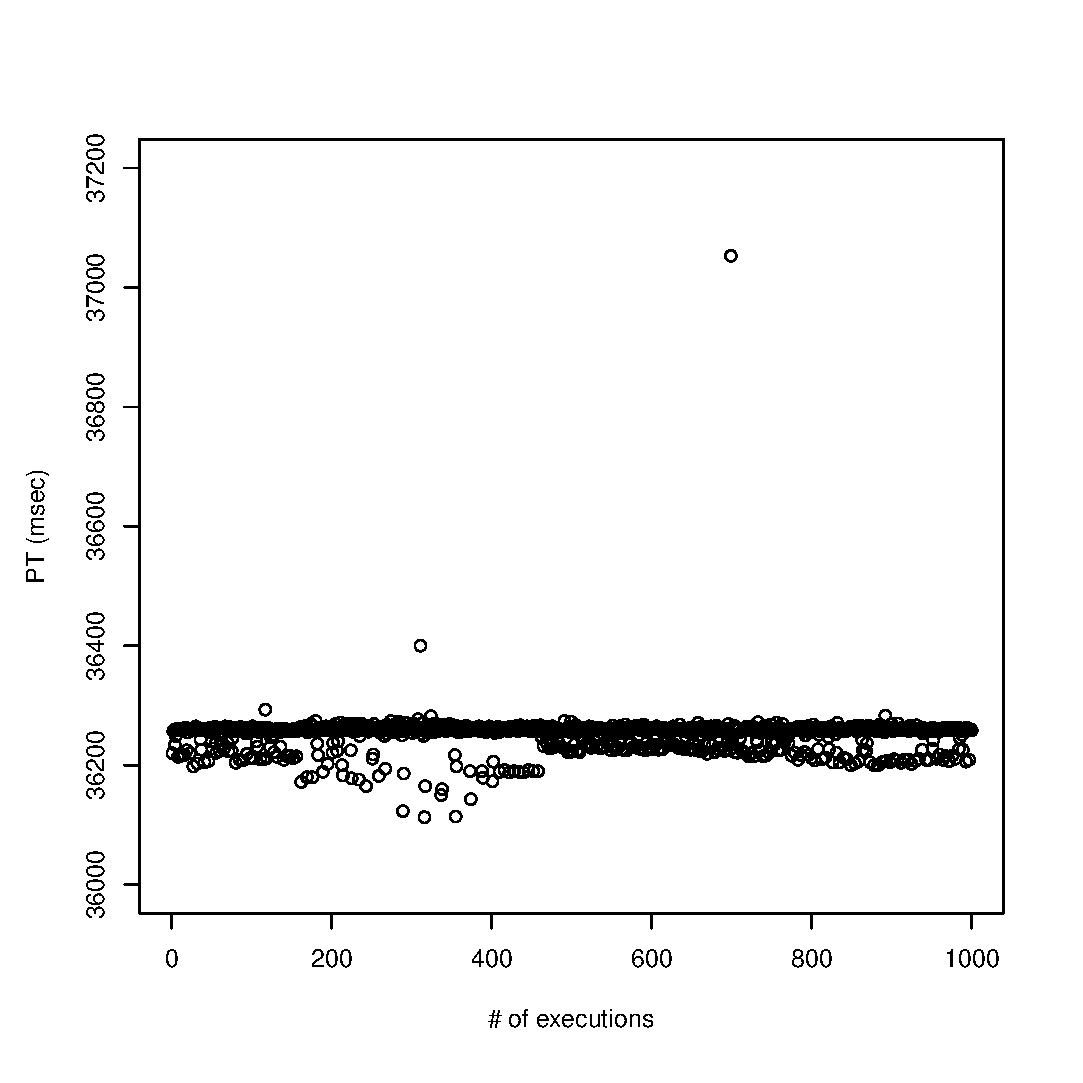
\includegraphics[scale=0.43]{figures/sodb8-ntp-on-turbo-off/32_sec_pt_all.eps}
		\label{fig:32_sec_pt_all}
	}
	\subfigure[Per-execution PT on PUT64]{
		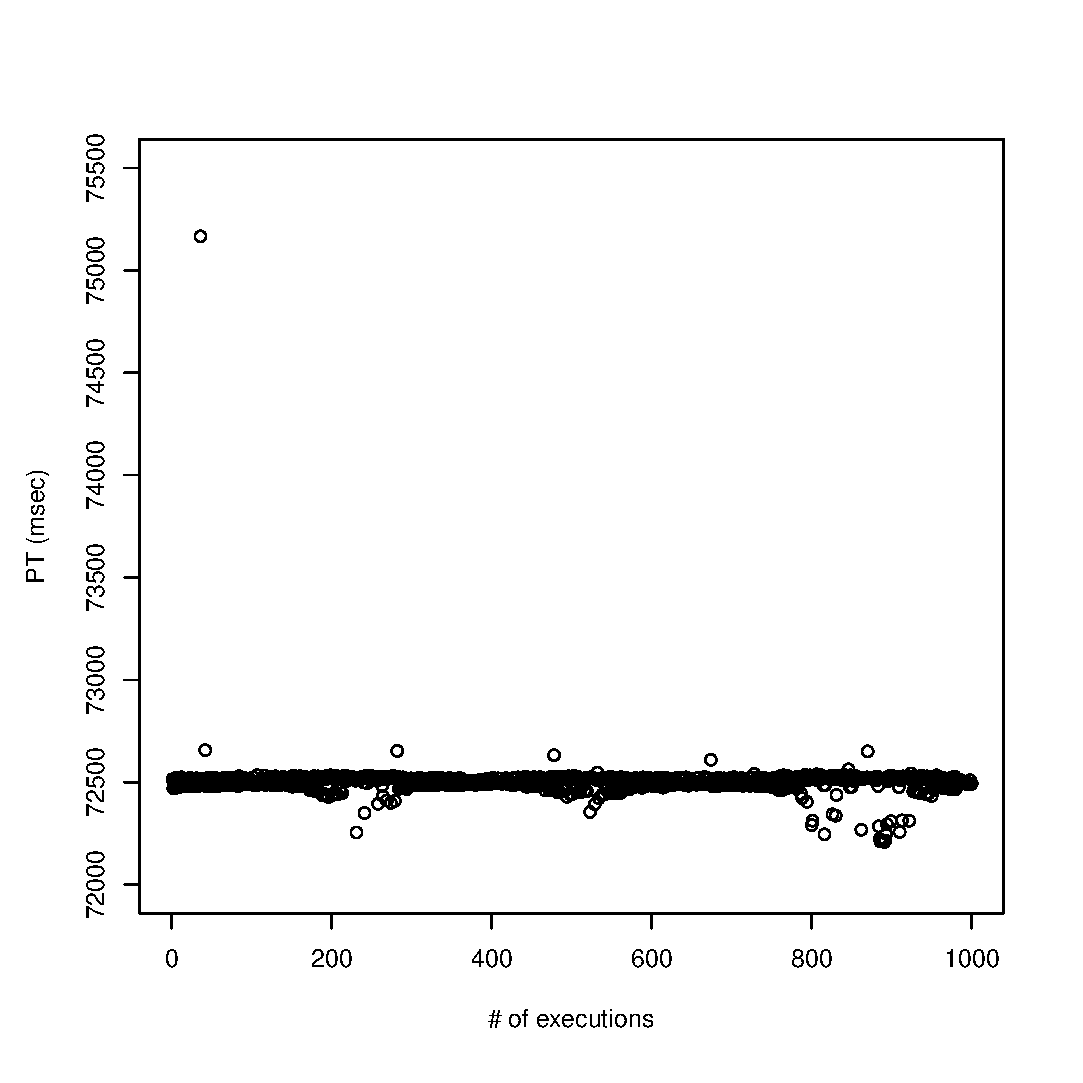
\includegraphics[scale=0.43]{figures/sodb8-ntp-on-turbo-off/64_sec_pt_all.eps}
		\label{fig:64_sec_pt_all}
	}
	\caption{Per-execution PT on PUT8, PUT16, PUT32, and PUT64~\label{fig:peak_pt}}
\end{figure}

There are three common things that we can draw regarding this phenomenon. 
First of all, literally all the peaks are far above the main band. 
Second, every experiment reveals a few peaks. 
Lastly, their occurrence does not have any periodic cycle. In other words, 
the outliers are scattered all over the places. 
It looks irregular and appears randomly at a specific execution.

\paragraph{Hypothesis} ``{\it The outliers could be correlated with processes 
scheduled to run at some point during our experiment.}''\\

%\paragraph{Hypothesis} ``{\it Considering that there could be processes that can be scheduled 
%during the experiment, these peaks could be correlated to this.}''
%
We looked at the data revealing the peaks in every experiment. 
Interestingly, {\em CPU\_COUNT}, representing \# of context swaps, is positively 
correlated with peak. PT grows linearly with the increase of \# of context switches. 
The correlation coefficient of PT and the context switches is 0.67, which is quite high. 
(The correlation between PT and \# of run processes is also positive.) 
Hence, this hypothesis is supported. 

\paragraph{Status} We have understood this.

\newpage

\subsection{Periodic Peaks in Frequency of PT}
 
\paragraph{Presumption} No peak except the median PT

\paragraph{Description} 
Figure~\ref{fig:pt_hist} shows the frequency of PT in the experiments 
whose respective expected running time is 4 and 8 seconds. 
This phenomenon indicates that a few peaks in frequency of PT are regularly seen. 
The phenomenon was observed from the EMPv2 data.

\begin{figure}[H]
	\centering
	\subfigure[PT frequency on PUT4]{
		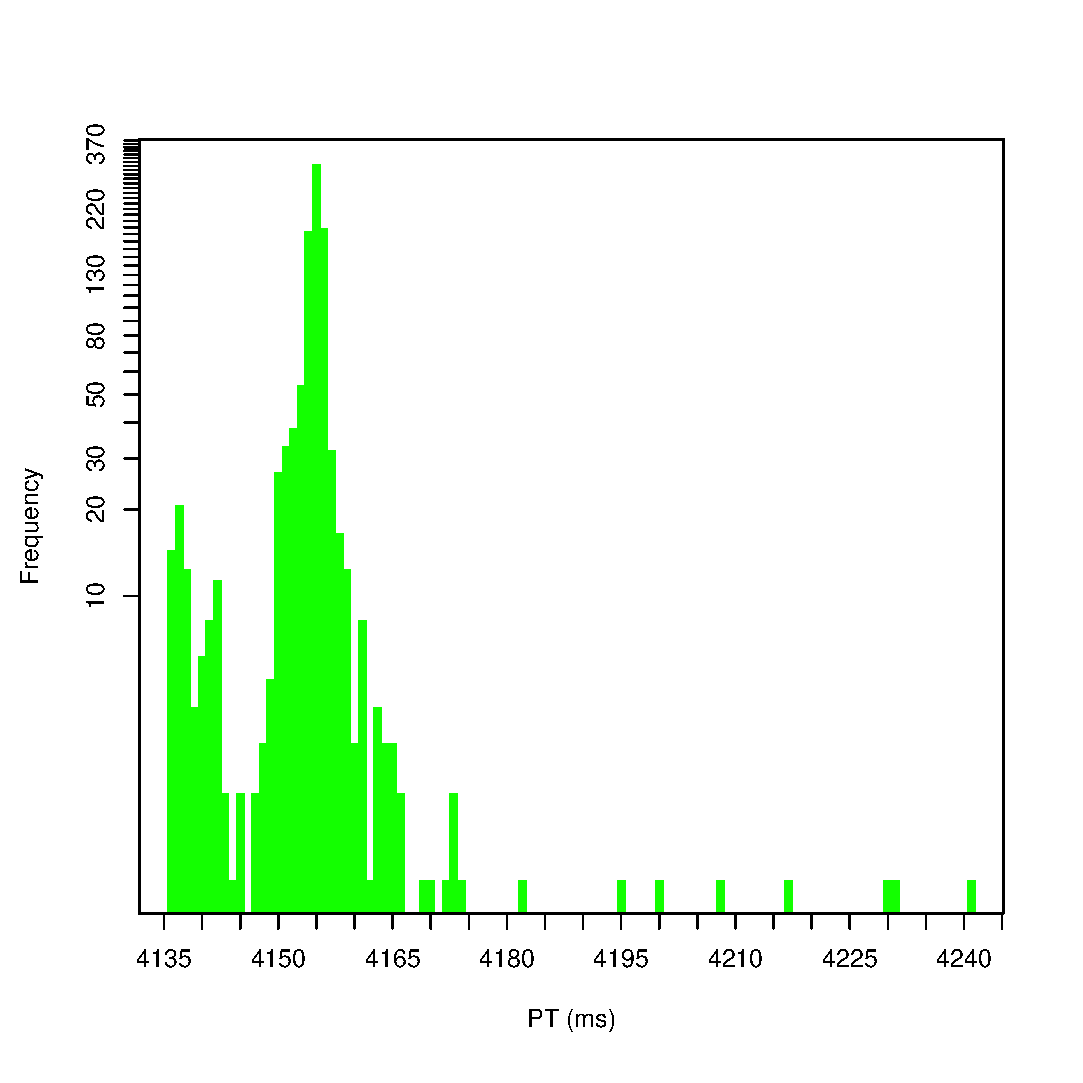
\includegraphics[scale=0.43]{figures/sodb8-ntp-on-turbo-on/4_sec_pt_hist.eps}
		\label{fig:4_sec_pt_hist}
	}
	\subfigure[PT frequency on PUT8]{
		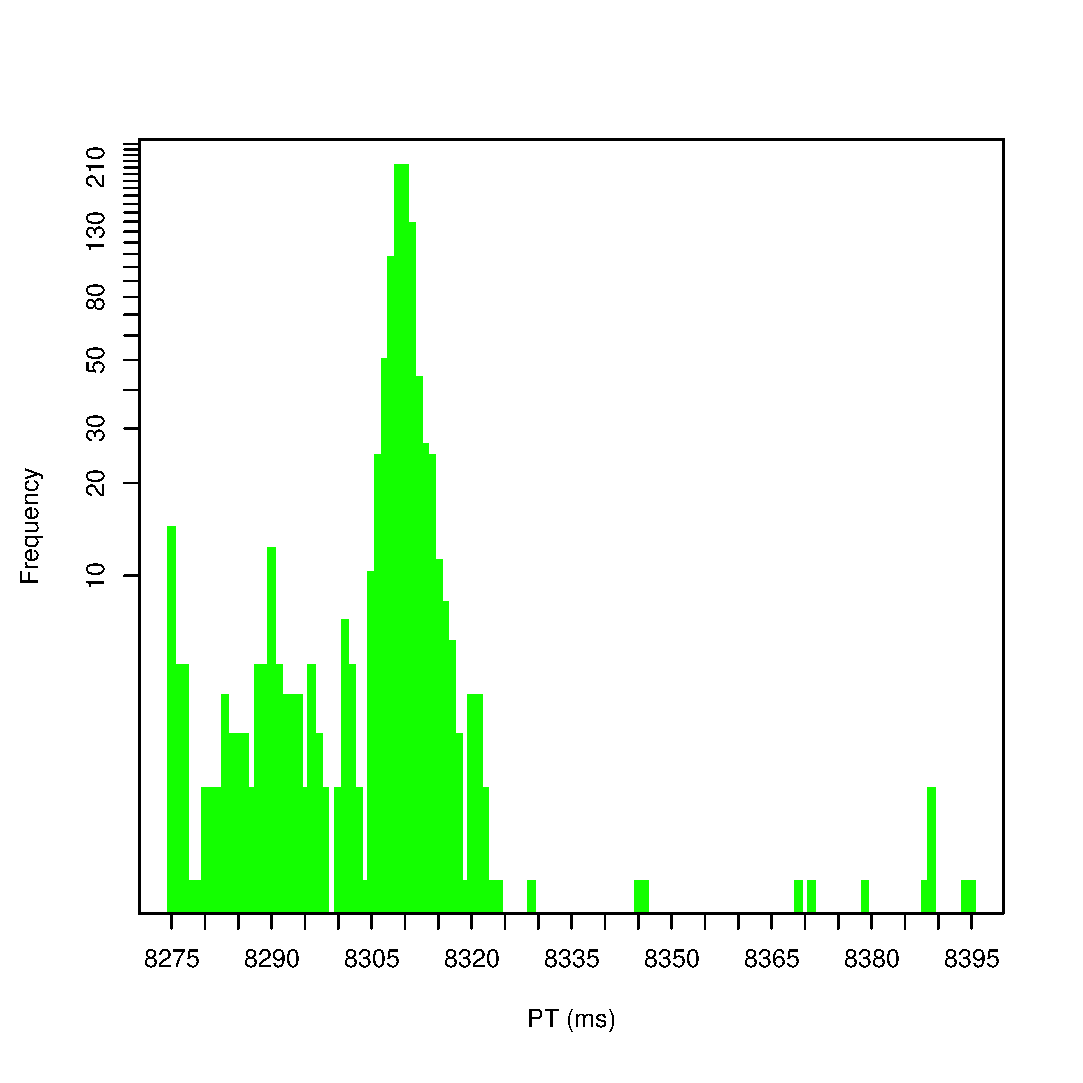
\includegraphics[scale=0.43]{figures/sodb8-ntp-on-turbo-on/8_sec_pt_hist.eps}
		\label{fig:8_sec_pt_hist}
	}
	\caption{PT frequency on PUT4 and PUT8~\label{fig:pt_hist}}
\end{figure}

\paragraph{Analysis} In Figure~\ref{fig:4_sec_pt_hist}, we could see two distinct peaks 
formed around 4,138 msecs and 4,142 msecs before the highest peak around 4,155 msecs. 
This pattern was also observed in Figure~\ref{fig:8_sec_pt_hist}, 
where there were about three peaks shown at 8,275 msecs, 8,292 msecs, and 8,300 msecs 
before the highest one around 8,318 msecs. 
The peaks appeared to repeat every around 8 msecs. 
This periodicty seems formed by the same PT values on PUT4 and PUT8. 
In particular, these PT values were below the median. 
The low PT values were calculated when PT periodically went down to the minimum, 
as discussed in Section~\ref{sec:pd_pt}. 
As a consequence, periodic peaks in frequency were observed, as illustrated in Figure~\ref{fig:pt_hist}. 

\paragraph{Hypothesis} ``{\it Heavier PUT will also have similar periodic peaks in frequency due to their low PT values.}'' 

\paragraph{Test} 
Such similar peaks in frequency periodically 
appeared in the measurements on PUT16 and PUT32, as depicted in Figure~\ref{fig:extra_pt_hist}. 
Again, EMPv2 was used for this test.

\begin{figure}[H]
	\centering
	\subfigure[PT frequency on PUT16]{
		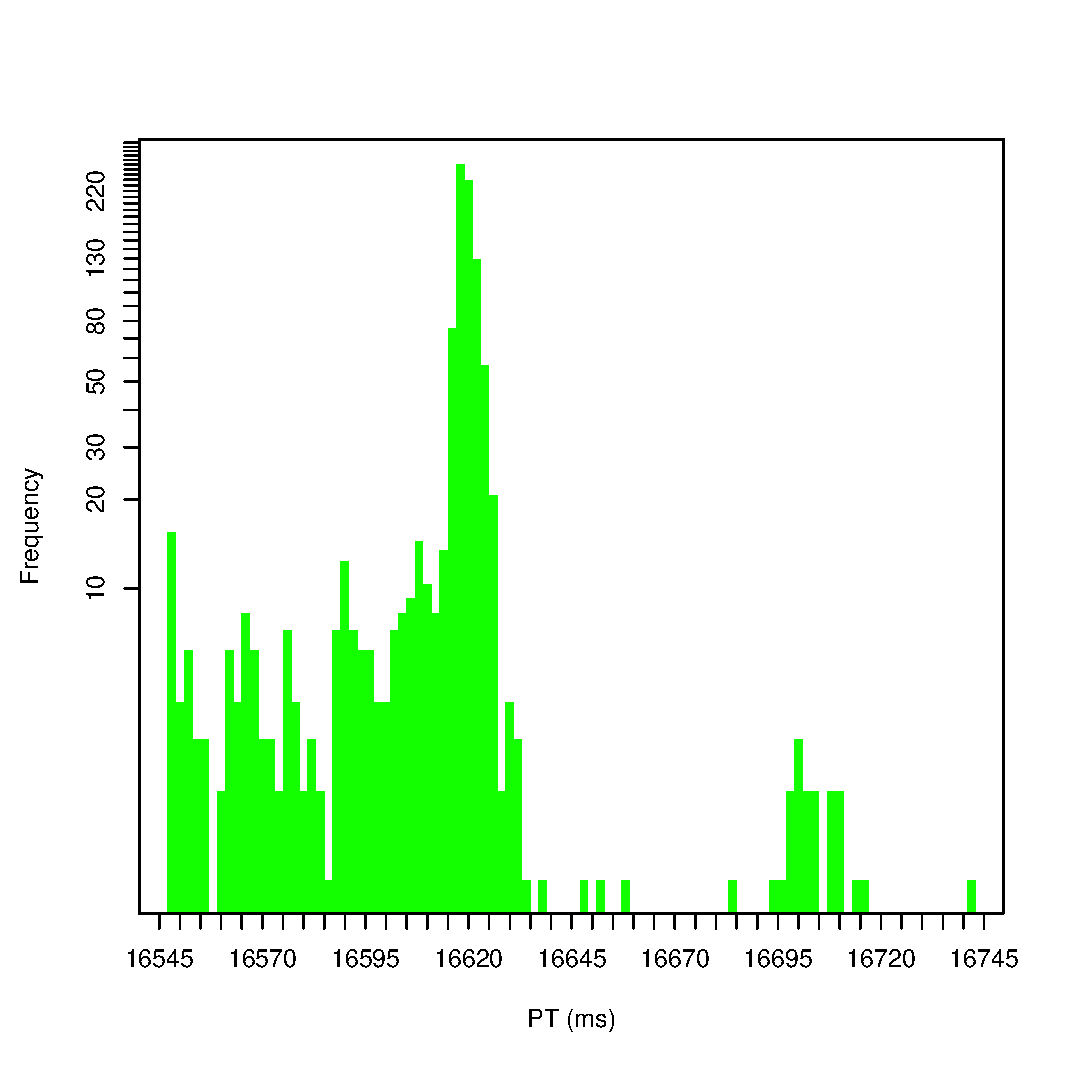
\includegraphics[scale=0.43]{figures/sodb8-ntp-on-turbo-on/16_sec_pt_hist.eps}
		\label{fig:16_sec_pt_hist}
	}
	\subfigure[PT frequency on PUT32]{
		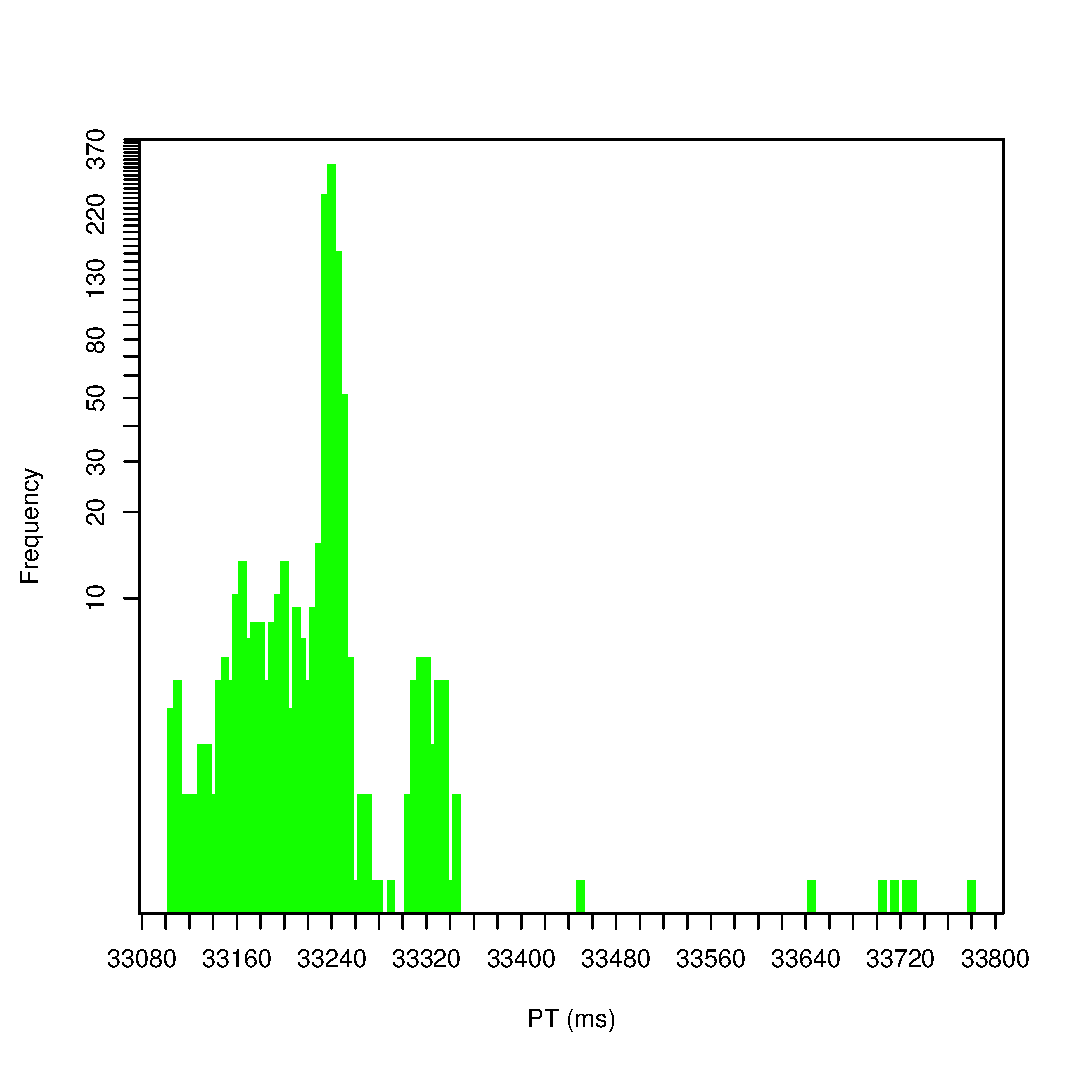
\includegraphics[scale=0.43]{figures/sodb8-ntp-on-turbo-on/32_sec_pt_hist.eps}
		\label{fig:32_sec_pt_hist}
	}
	\caption{PT frequency on PUT16 and PUT32~\label{fig:extra_pt_hist}}
\end{figure}

Therefore, this hypothesis is supported. 

\paragraph{Status} The cause is understood.

\newpage

\subsection{Increasing Minimum and Maximum Difference in PT}
%Figure~\ref{fig:mm_pt_dist} shows the distance between the minimum and maximum PT 
%over increasing amount of work. 

\paragraph{Presumption} Almost zero or very small constant

\paragraph{Description} 
This phenomenon indicates that the difference between the maximum and minimum of the measured PT values 
grows linearly over increasing task length, as shown in Figure~\ref{fig:mm_pt_dist}. 
Note that $xy$ axes are in log scale. 
This phenomenon was observed from the EMPv2 data.

% 60 =  1.778 => 0.058
% 89 = 1.9493 => 0.043
% 106 = 2.02  => 0.025
% 121 = 2.08  => 0.0146
% 195 = 2.29  => 0.0117
% 770 = 2.89  => 0.023
% 1038 = 3.01 => 0.0156

\begin{figure}[H]
\centering
\includegraphics[scale=0.8]{figures/sodb8-ntp-on-turbo-on/overall_pt_diff.eps}
\caption{Increasing difference over increasing task length~\label{fig:mm_pt_dist}}
\end{figure}

\paragraph{Analysis} As task length increases, the PT difference increases. 
Considering that the $y$-axis values are plotted in log scale, the difference grows linearly. 
It appears to be synchronized with the degree of increasing task length. 
Our expectation on PT was flat, and thus, the increasing difference was strange. 

\paragraph{Hypothesis} ?

\paragraph{Test} ?


%\paragraph{Hypothesis} ``{\it Disabling the Turbo mode will show the flat PT difference.}''
%
%\paragraph{Test} Figure~\ref{fig:off_turbo_pt_dist} shows the PT difference when the Turbo mode was off.
%
%\begin{figure}[hp!]
%\centering
%\includegraphics[scale=0.9]{figures/turbo_mode/overall_pt_diff.eps}
%\caption{PT difference over increasing expected running time under the disabled Turbo mode\label{fig:off_turbo_pt_dist}}
%\end{figure}
%
%Unfortunately, overall the PT difference still grows over increasing expected running time even 
%after the mode was not enabled. It went down at the four-second task, compared to that of the two-second task. 
%However, the increase is still shown.

%\paragraph{Hypothesis} ``{\it Even if we increase the expected running time of PUT,
%the difference in PT will be constant.}''
%
%Based on our expectation that PT should be flat, we anticipated that 
%the minimum and maximum PT through 1000 executions did not differ much, regardless of how long PUT took. 
%However, we observed that the difference got bigger over increasing the degree of the task. 
%For instance, the difference started with 60 msecs in the one-second task. 
%As the expected running times increase, the difference also grows somewhat linearly. 
%The difference reaches up to around 1040 msecs in the sixty-four second work. 
%Thus, the hypothesis is not supported. 
%
\paragraph{Status} Not understood.
%
%\subsection{Miscellaneous}
%
%\begin{enumerate}
%\item Note that the X-axis in th
%\end{enumerate}
%
%
\vspace{-0.01in}

\newpage

\section{Exploring a Proper Distribution for Measured Data}

Figures~\ref{fig:extra_pt_hist1},~\ref{fig:extra_pt_hist2},~\ref{fig:extra_pt_hist3},~\ref{fig:extra_pt_hist4},~\ref{fig:extra_pt_hist5},~\ref{fig:extra_pt_hist6}, 
and~\ref{fig:extra_pt_hist7} represent the histograms of ET and PT on the 1 $\sim$ 4096 second tasks. 
Nnormal and beta distributions are fitted on the histograms as well.
For these histograms, we used EMPv5, which identified and removed outliers in its measurements.

\begin{figure}[H]
	\centering
	\subfigure[ET frequency on PUT1]{
		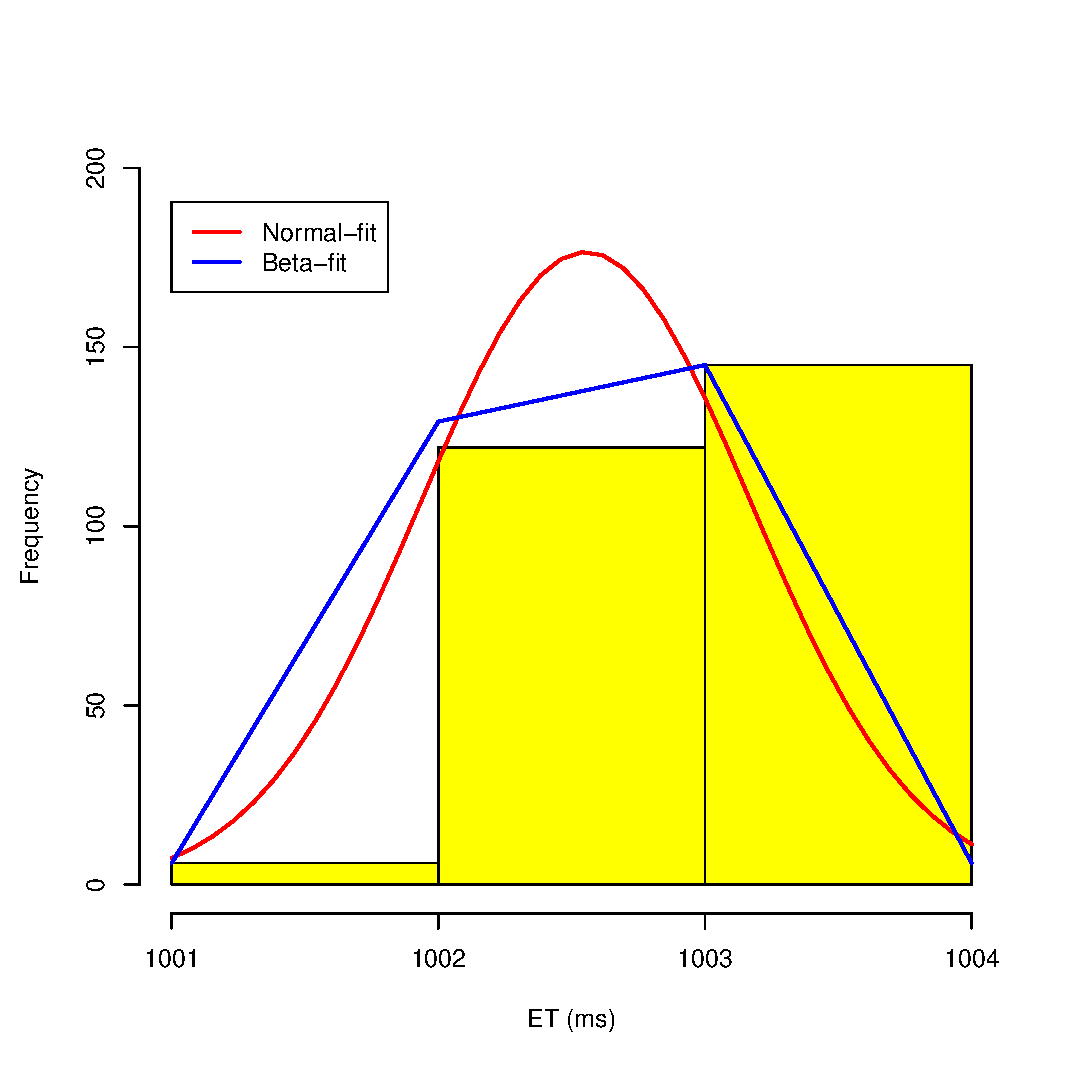
\includegraphics[scale=0.43]{figures/sodb12-ntp-on-turbo-off/1_sec_et_hist.eps}
		\label{fig:1_sec_et_hist1}
	}
	\subfigure[PT frequency on PUT1]{
		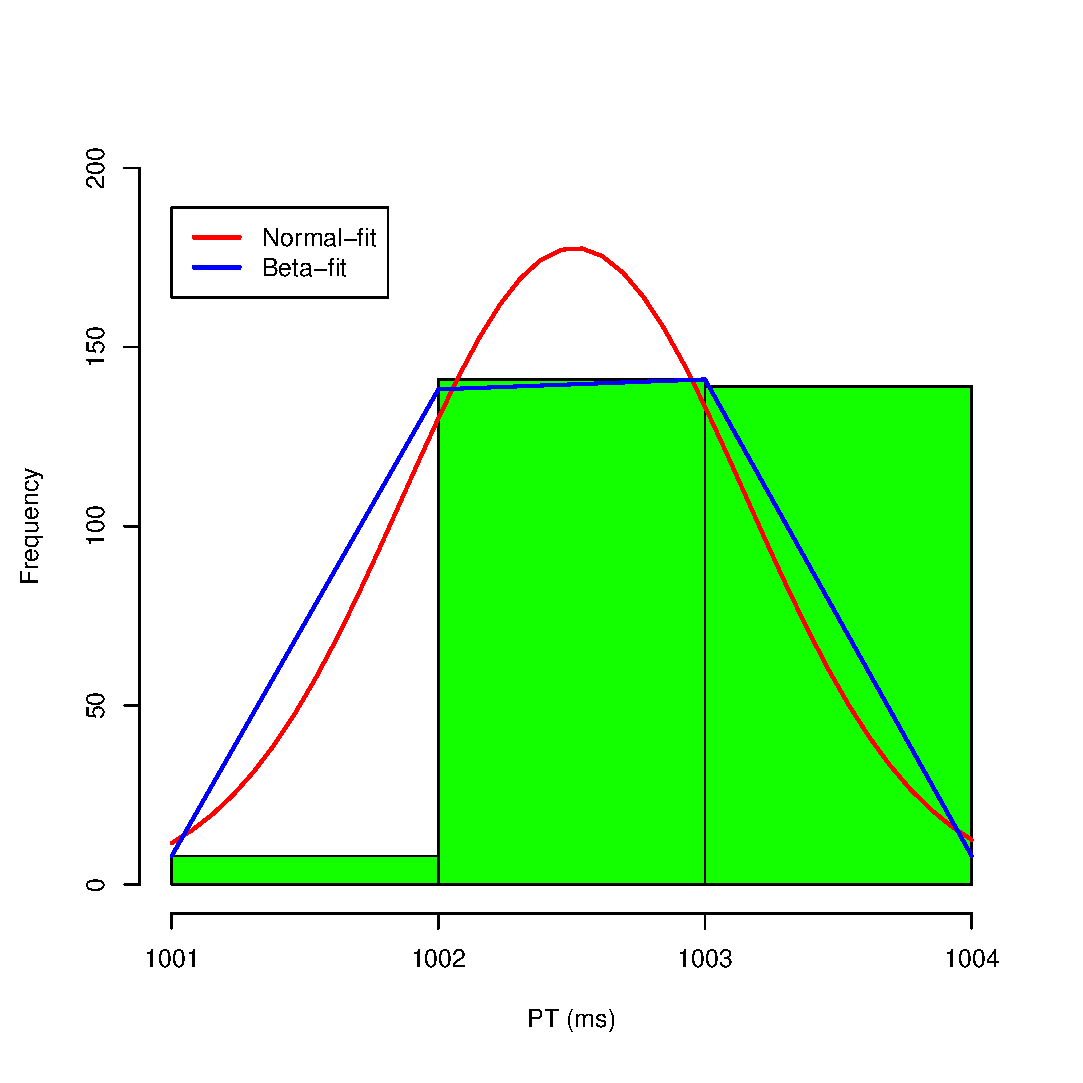
\includegraphics[scale=0.43]{figures/sodb12-ntp-on-turbo-off/1_sec_pt_hist.eps}
		\label{fig:1_sec_pt_hist1}
	}
	\subfigure[ET frequency on PUT2]{
		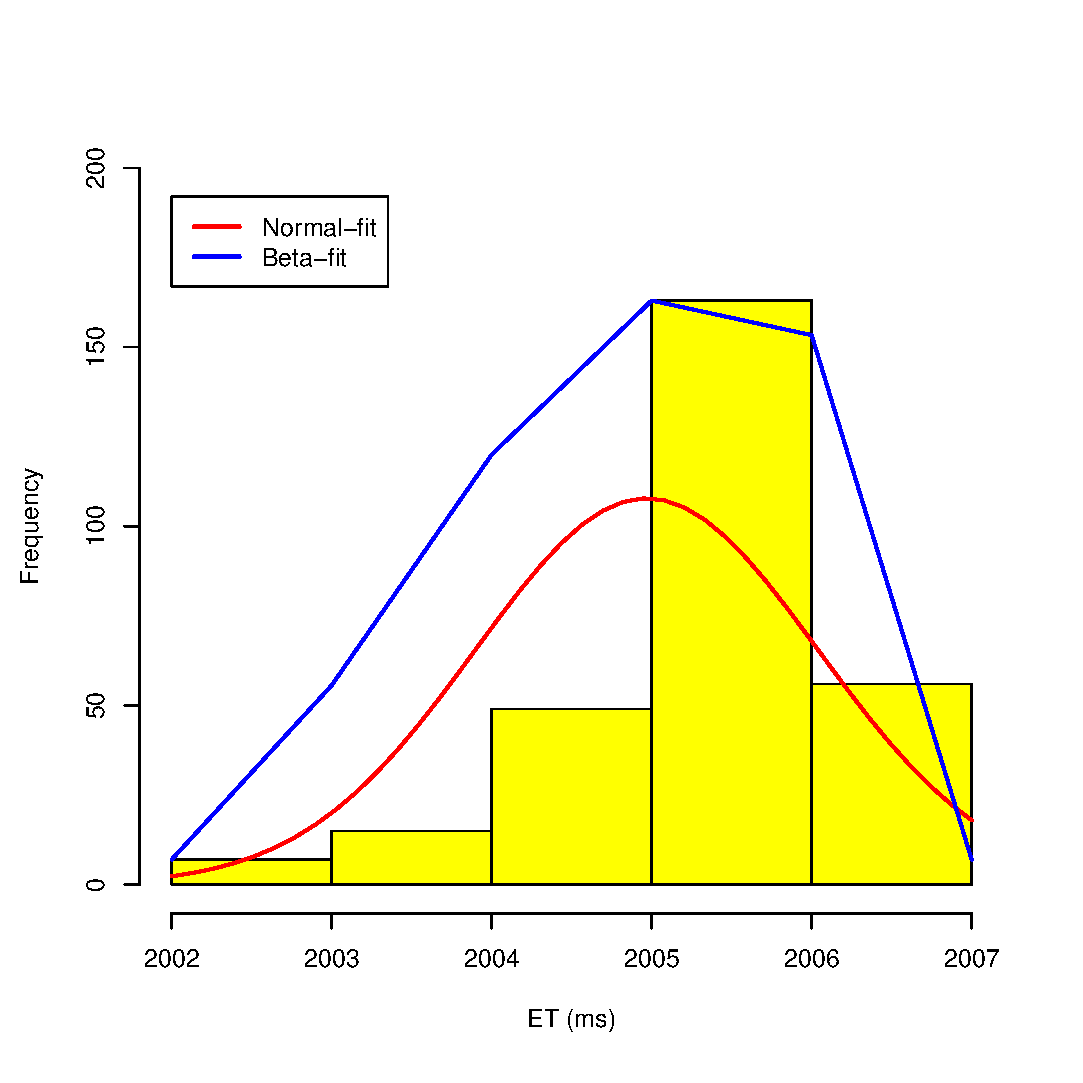
\includegraphics[scale=0.43]{figures/sodb12-ntp-on-turbo-off/2_sec_et_hist.eps}
		\label{fig:2_sec_et_hist1}
	}
	\subfigure[PT frequency on PUT2]{
		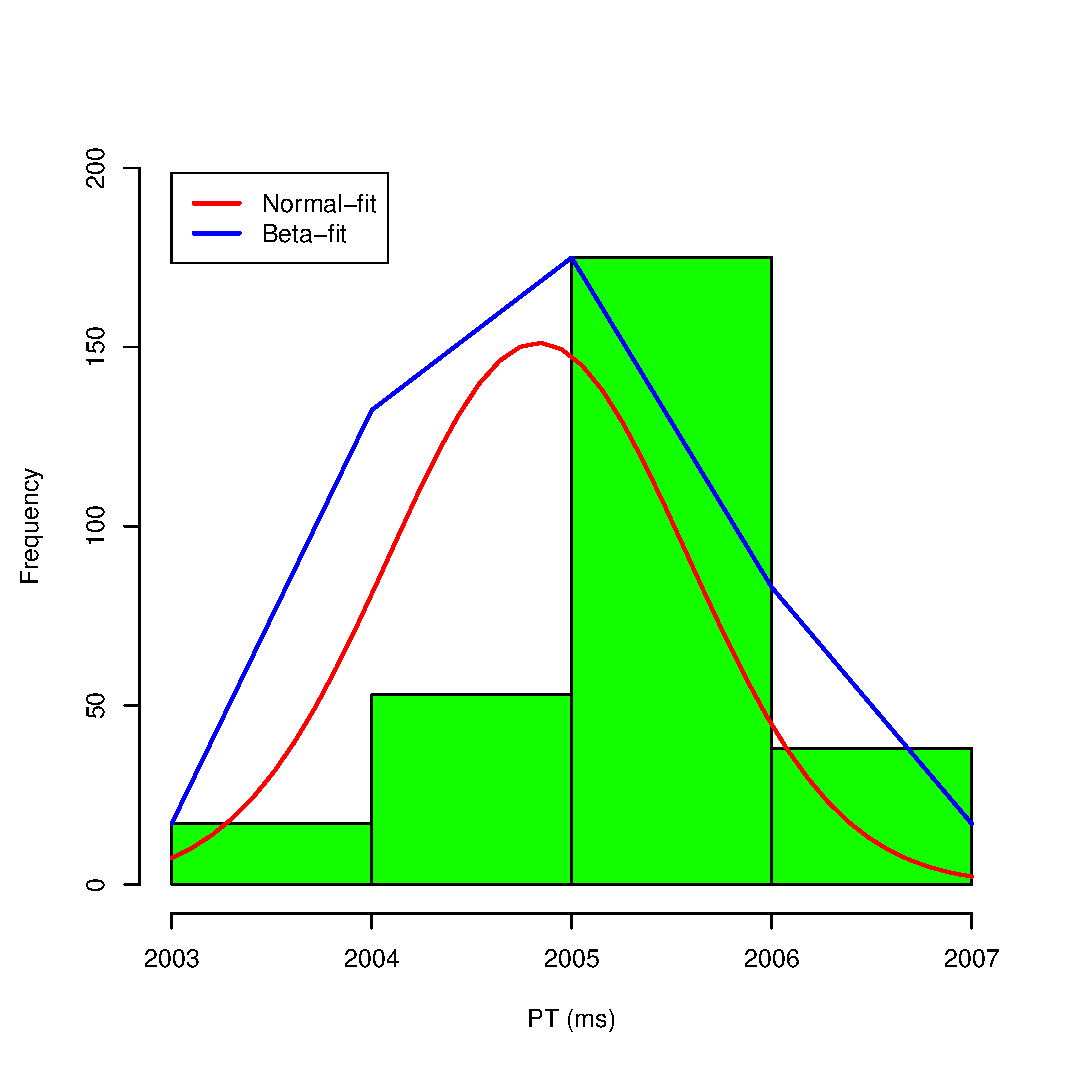
\includegraphics[scale=0.43]{figures/sodb12-ntp-on-turbo-off/2_sec_pt_hist.eps}
		\label{fig:2_sec_pt_hist1}
	}
	\caption{Normal and beta distributions fitting onto the histograms of the measurements of PUT1 and PUT2~\label{fig:extra_pt_hist1}}
\end{figure}

\begin{figure}[H]
	\centering
	\subfigure[ET frequency on PUT4]{
		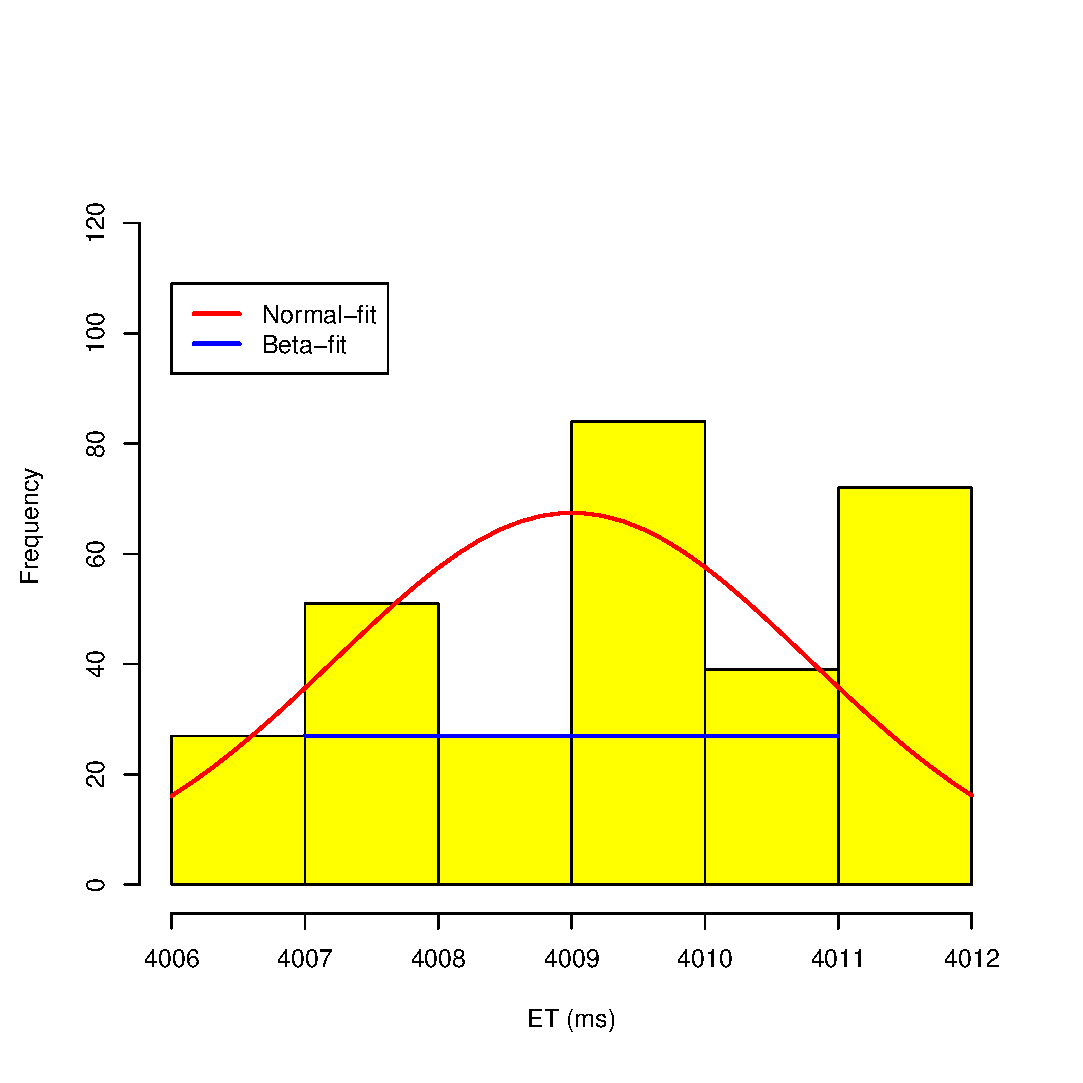
\includegraphics[scale=0.43]{figures/sodb12-ntp-on-turbo-off/4_sec_et_hist.eps}
		\label{fig:4_sec_et_hist1}
	}
	\subfigure[PT frequency on PUT4]{
		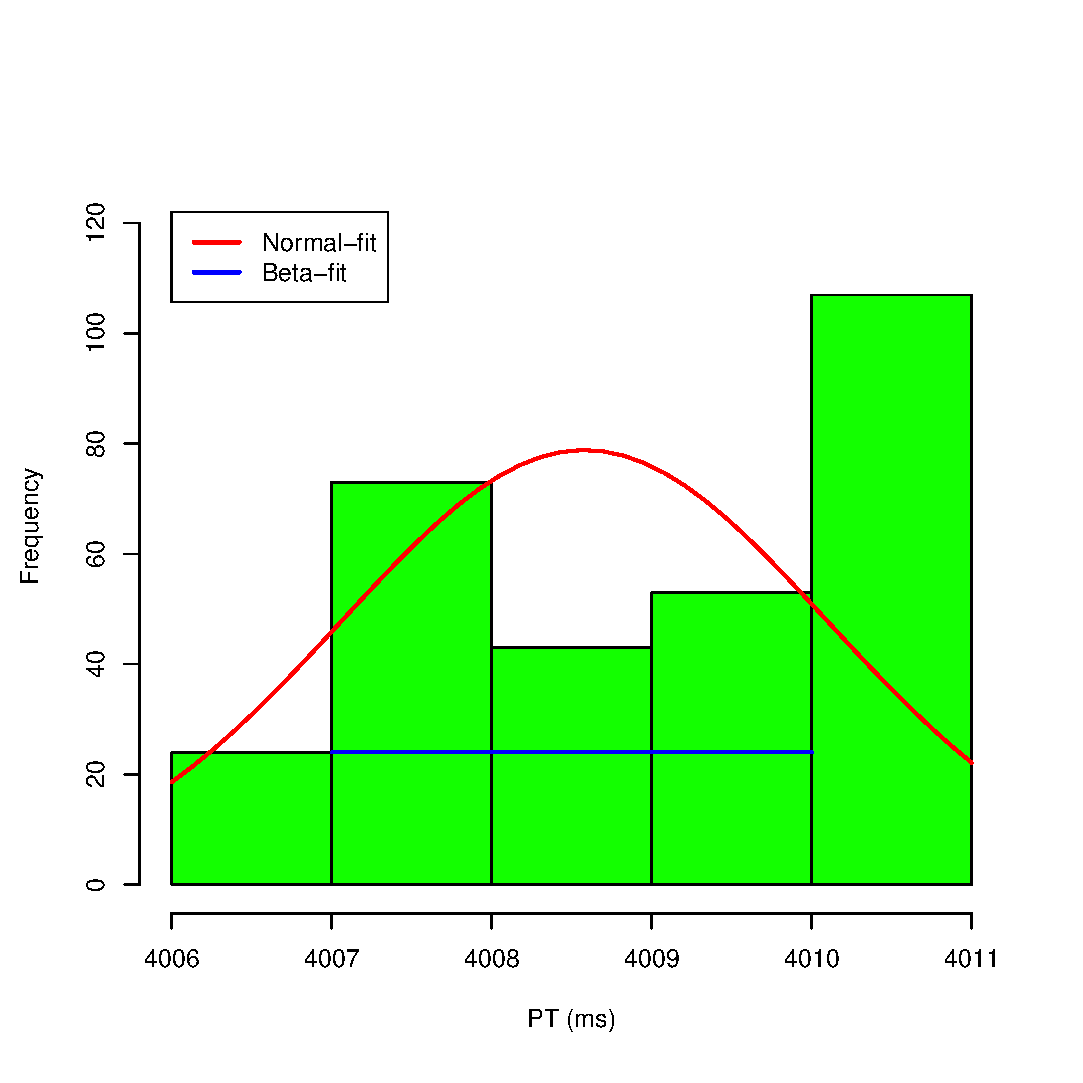
\includegraphics[scale=0.43]{figures/sodb12-ntp-on-turbo-off/4_sec_pt_hist.eps}
		\label{fig:4_sec_pt_hist1}
	}
	\subfigure[ET frequency on PUT8]{
		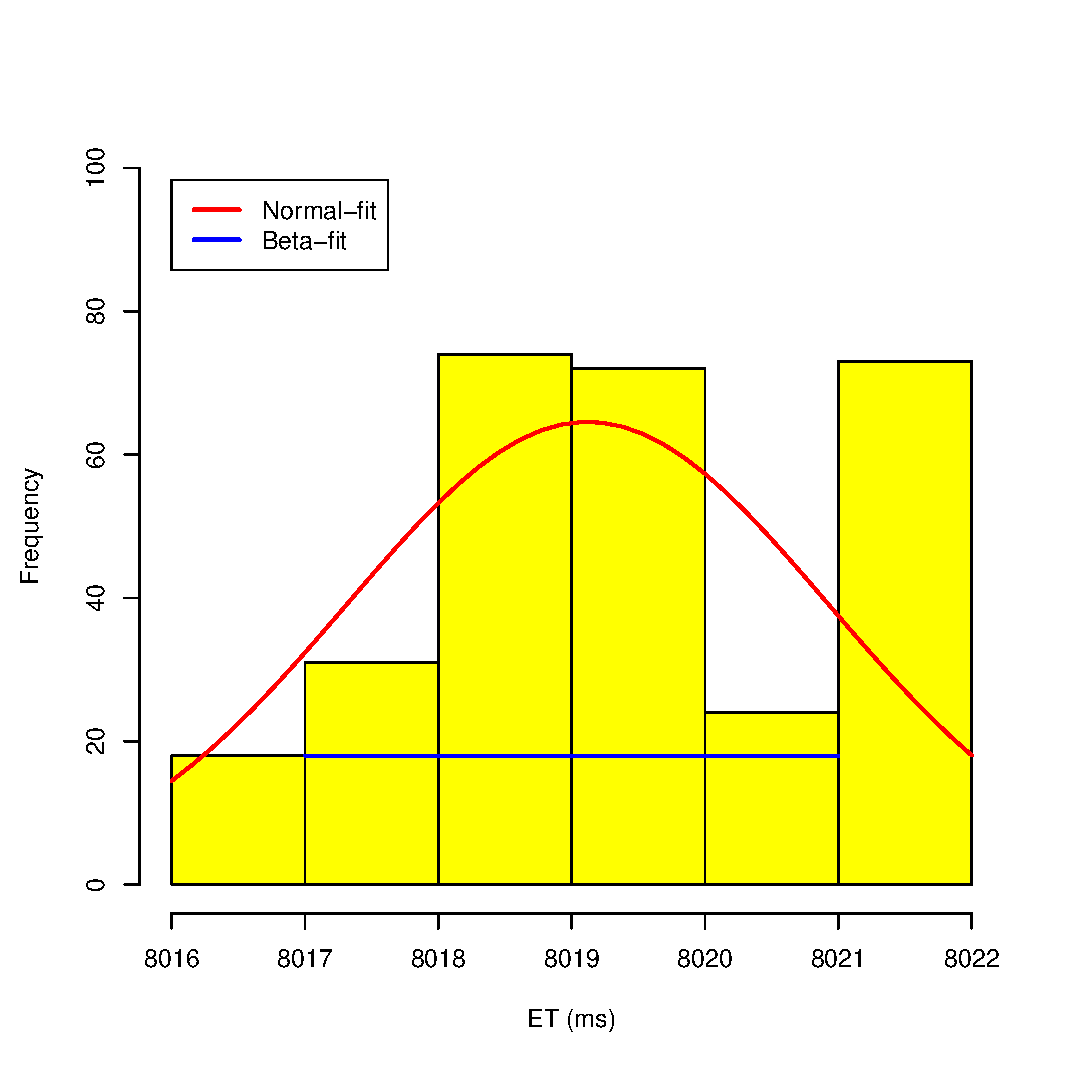
\includegraphics[scale=0.43]{figures/sodb12-ntp-on-turbo-off/8_sec_et_hist.eps}
		\label{fig:8_sec_et_hist1}
	}
	\subfigure[PT frequency on PUT8]{
		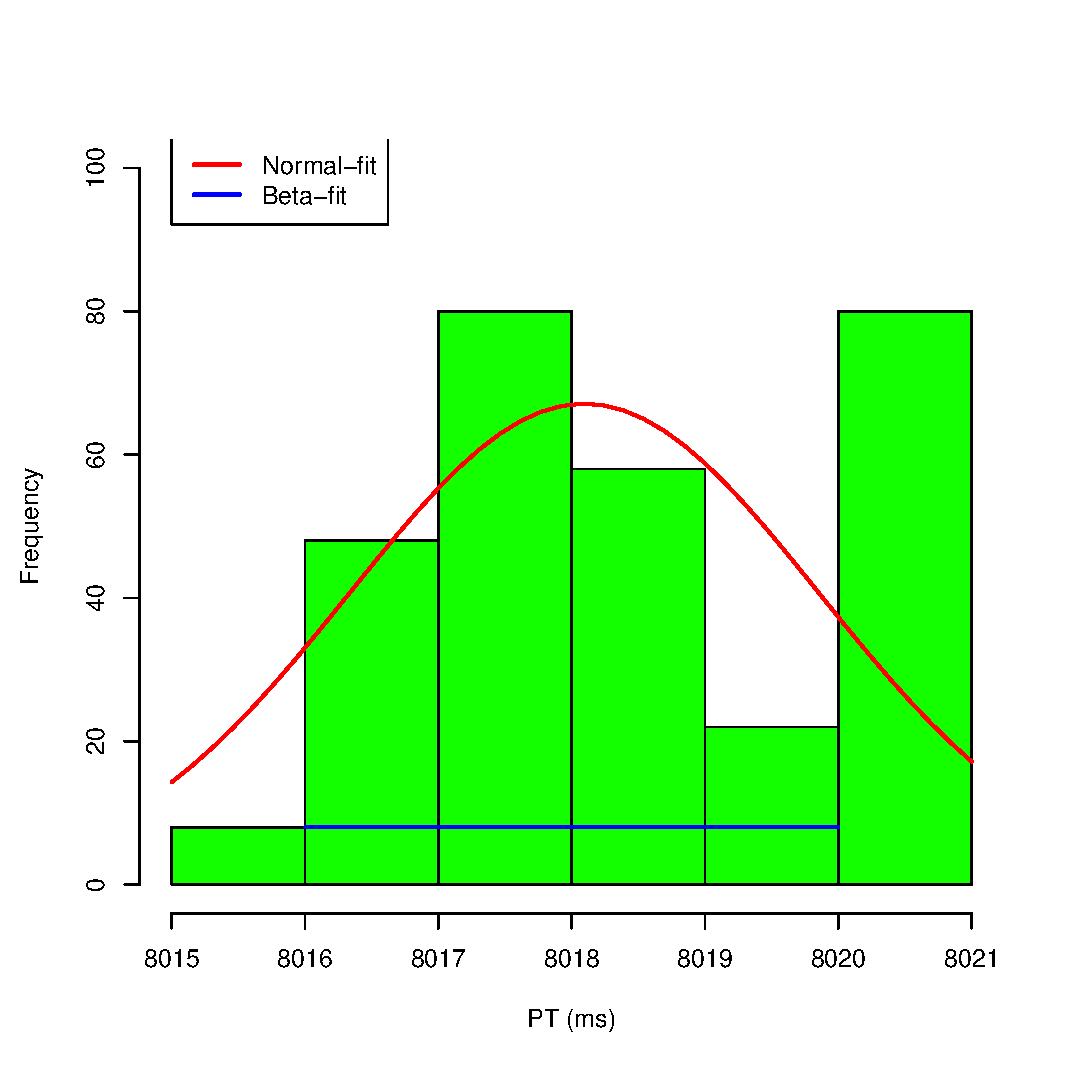
\includegraphics[scale=0.43]{figures/sodb12-ntp-on-turbo-off/8_sec_pt_hist.eps}
		\label{fig:8_sec_pt_hist1}
	}
	\caption{Normal and beta distributions fitting onto the histograms of the measurements of PUT4 and PUT8~\label{fig:extra_pt_hist2}}
\end{figure}

\begin{figure}[H]
	\centering
	\subfigure[ET frequency on PUT16]{
		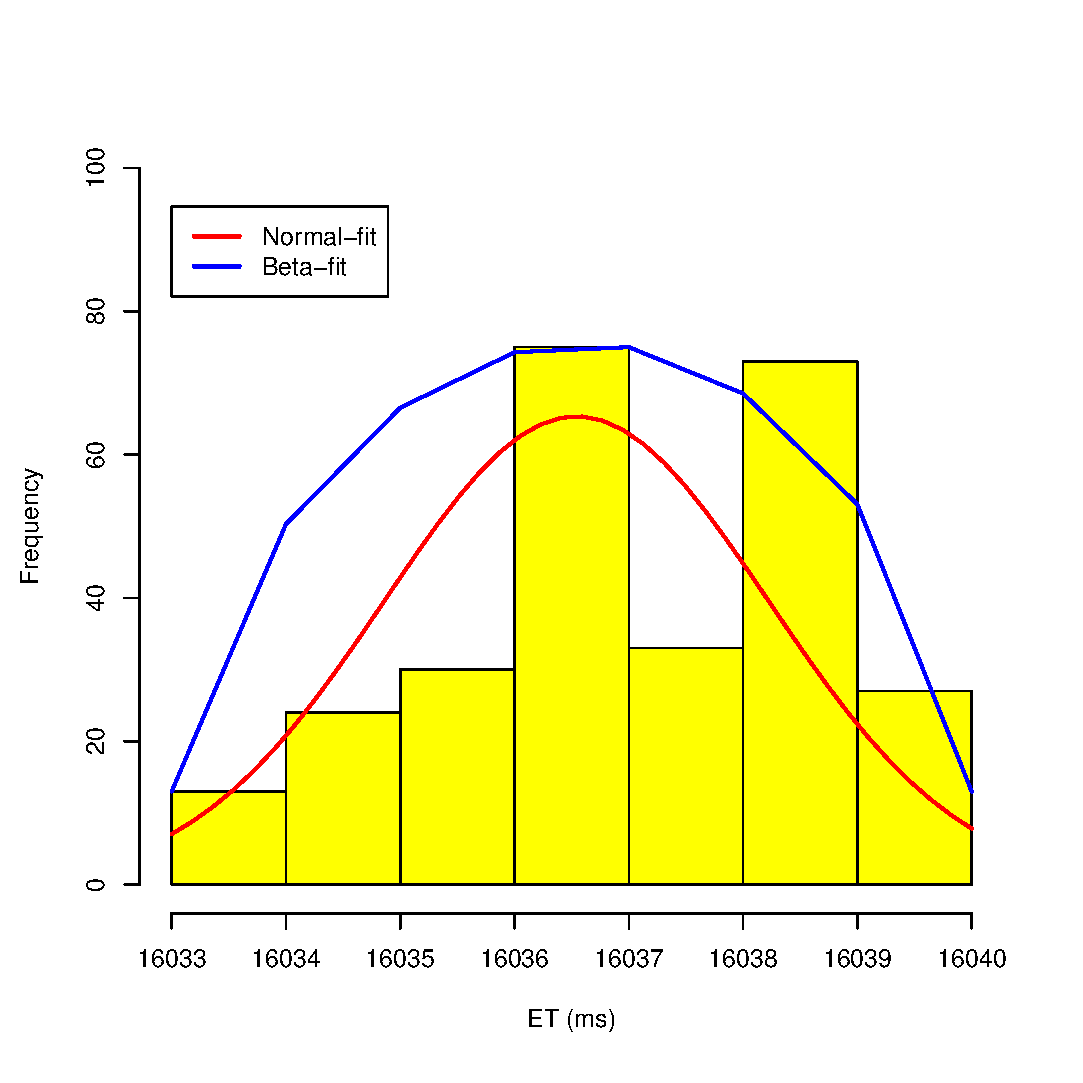
\includegraphics[scale=0.43]{figures/sodb12-ntp-on-turbo-off/16_sec_et_hist.eps}
		\label{fig:16_sec_et_hist1}
	}
	\subfigure[PT frequency on PUT16]{
		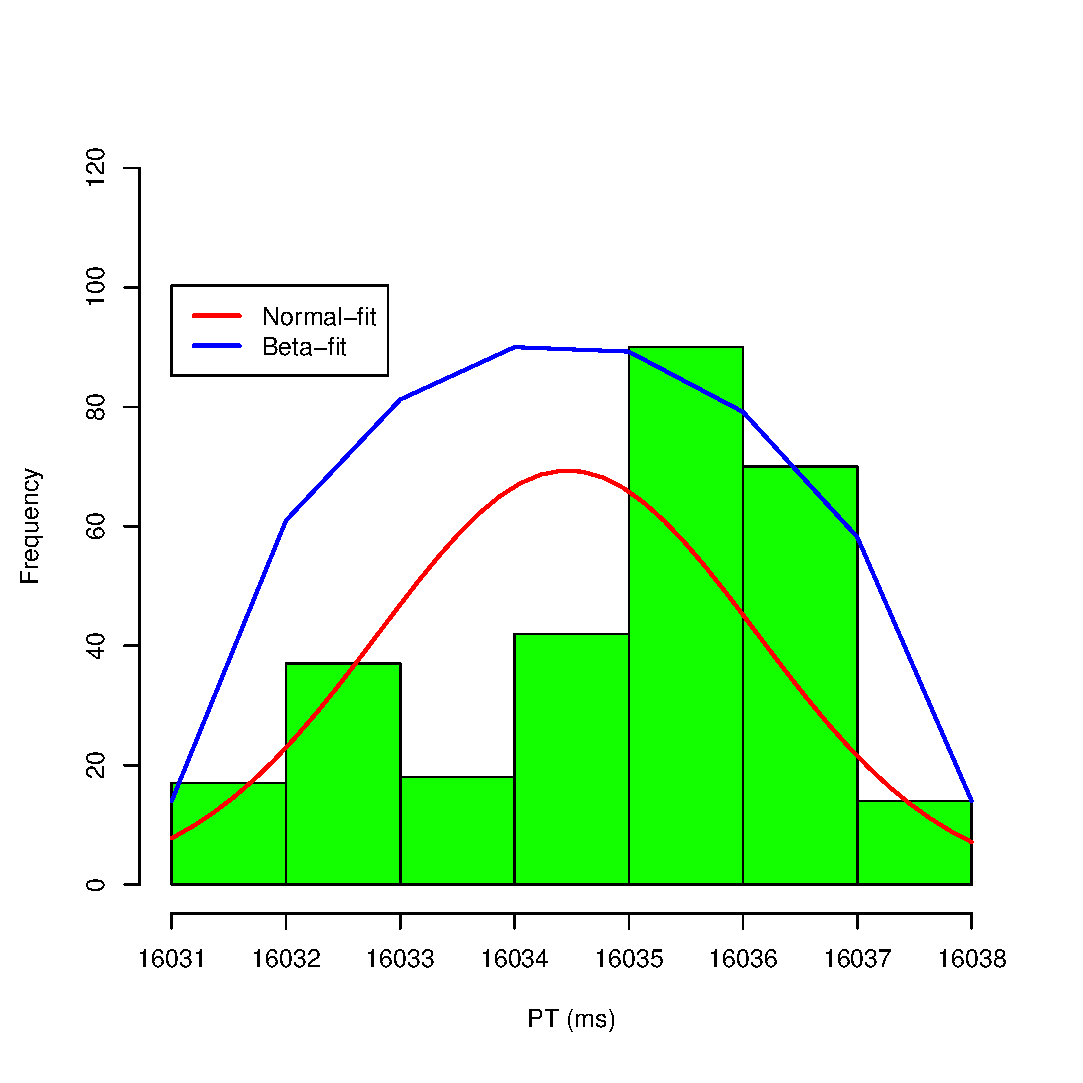
\includegraphics[scale=0.43]{figures/sodb12-ntp-on-turbo-off/16_sec_pt_hist.eps}
		\label{fig:16_sec_pt_hist1}
	}
	\subfigure[ET frequency on PUT32]{
		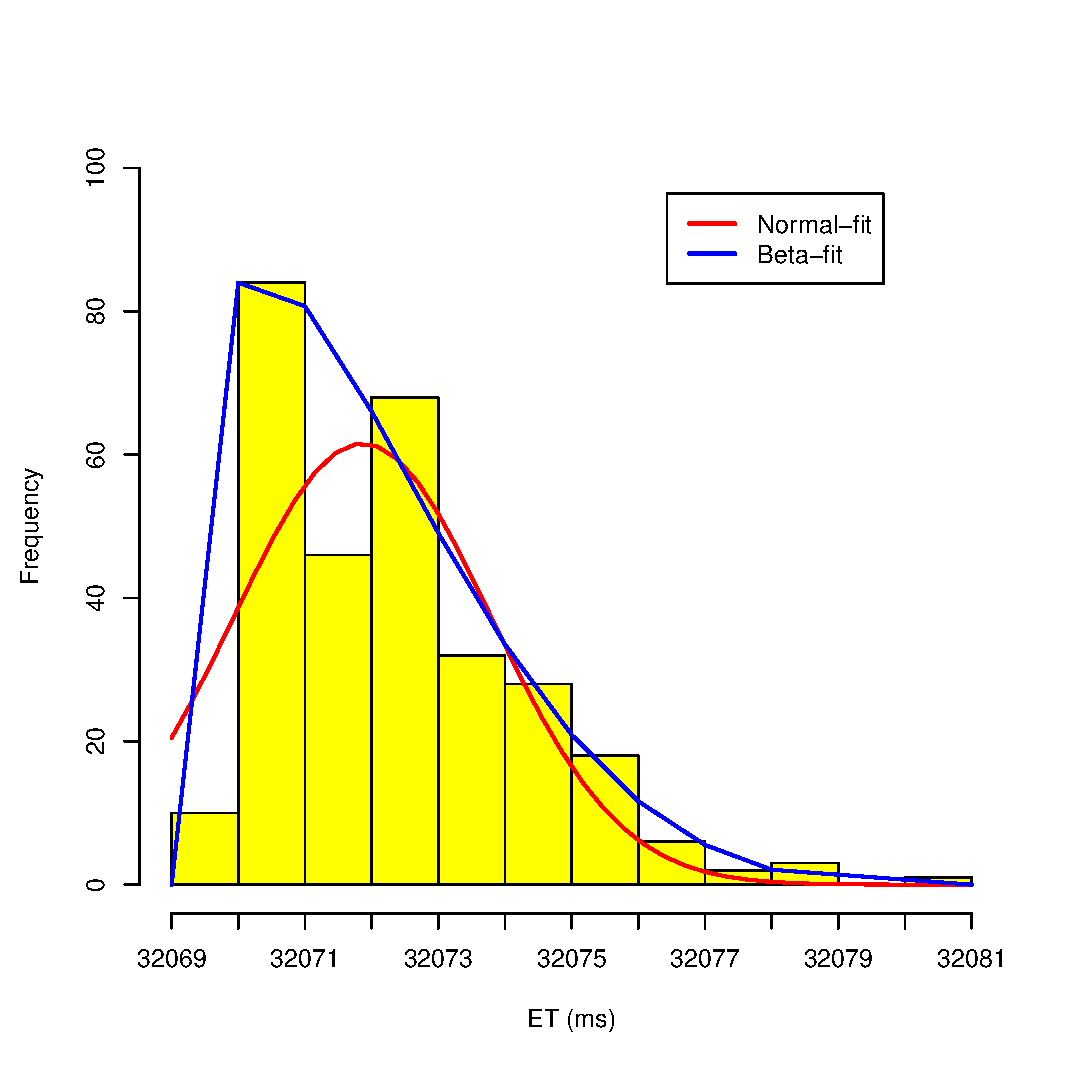
\includegraphics[scale=0.43]{figures/sodb12-ntp-on-turbo-off/32_sec_et_hist.eps}
		\label{fig:32_sec_et_hist1}
	}
	\subfigure[PT frequency on PUT32]{
		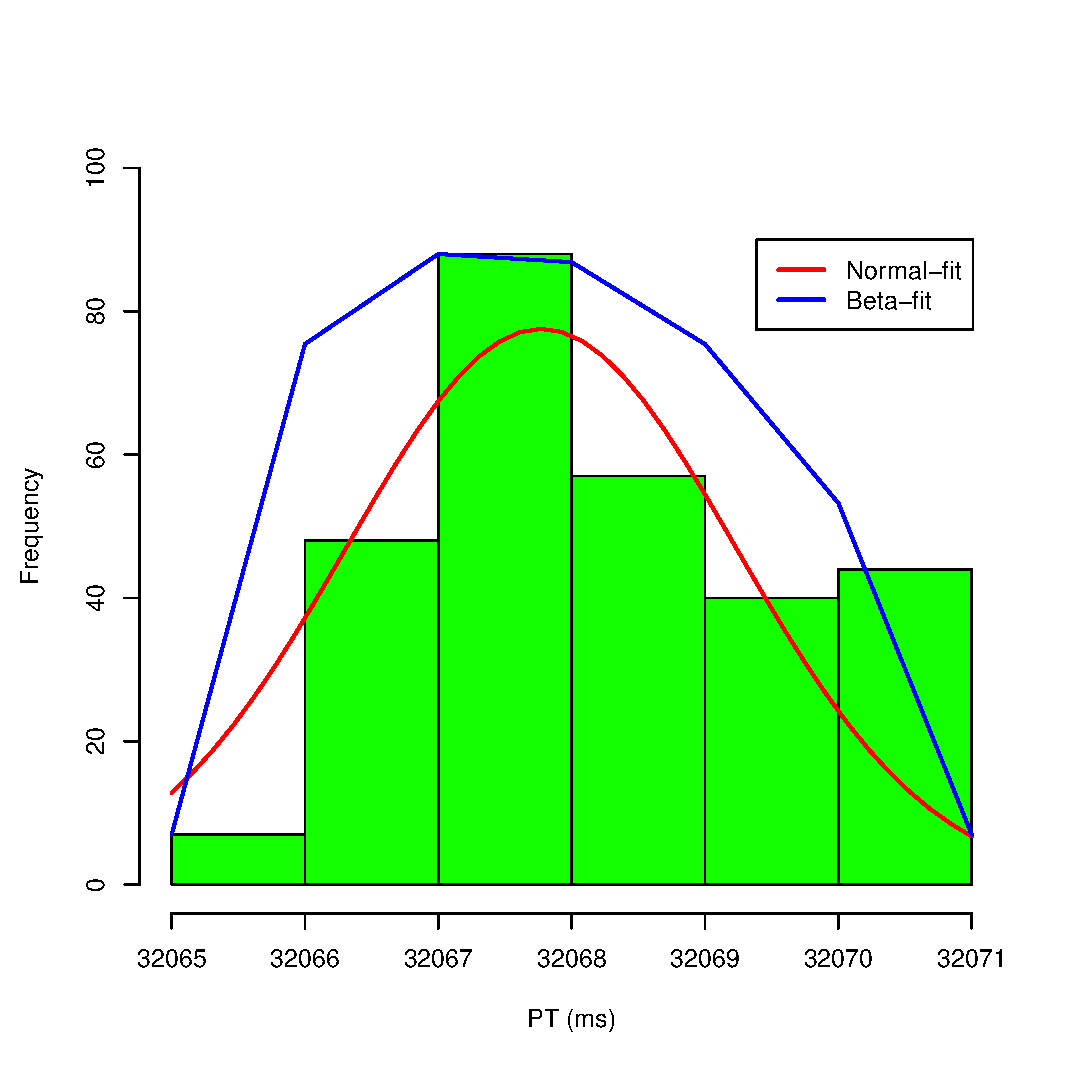
\includegraphics[scale=0.43]{figures/sodb12-ntp-on-turbo-off/32_sec_pt_hist.eps}
		\label{fig:32_sec_pt_hist1}
	}
	\caption{Normal and beta distributions fitting onto the histograms of the measurements of PUT16 and PUT32~\label{fig:extra_pt_hist3}}
\end{figure}

\begin{figure}
	\centering
	\subfigure[ET frequency on PUT64]{
		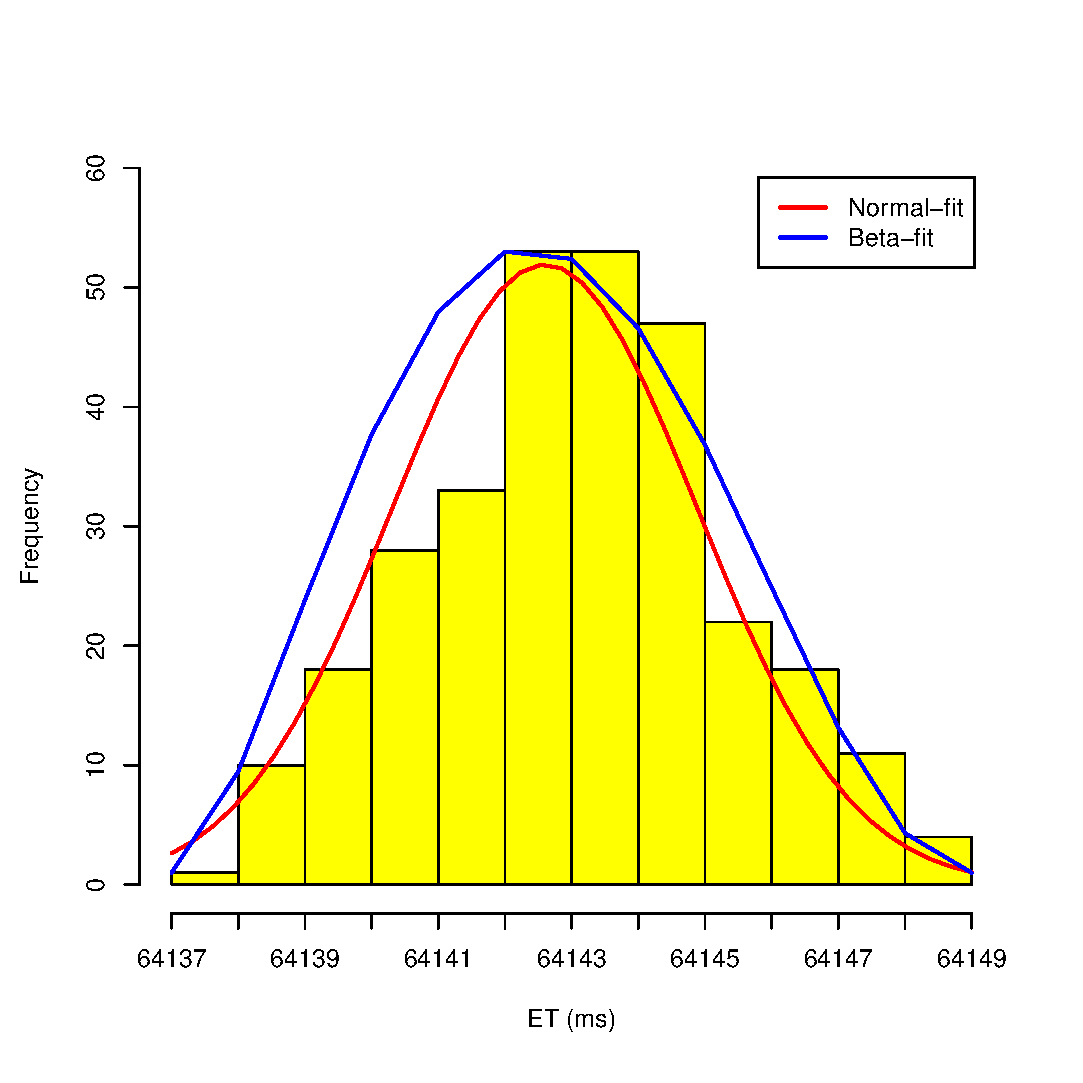
\includegraphics[scale=0.43]{figures/sodb12-ntp-on-turbo-off/64_sec_et_hist.eps}
		\label{fig:64_sec_et_hist1}
	}
	\subfigure[PT frequency on PUT64]{
		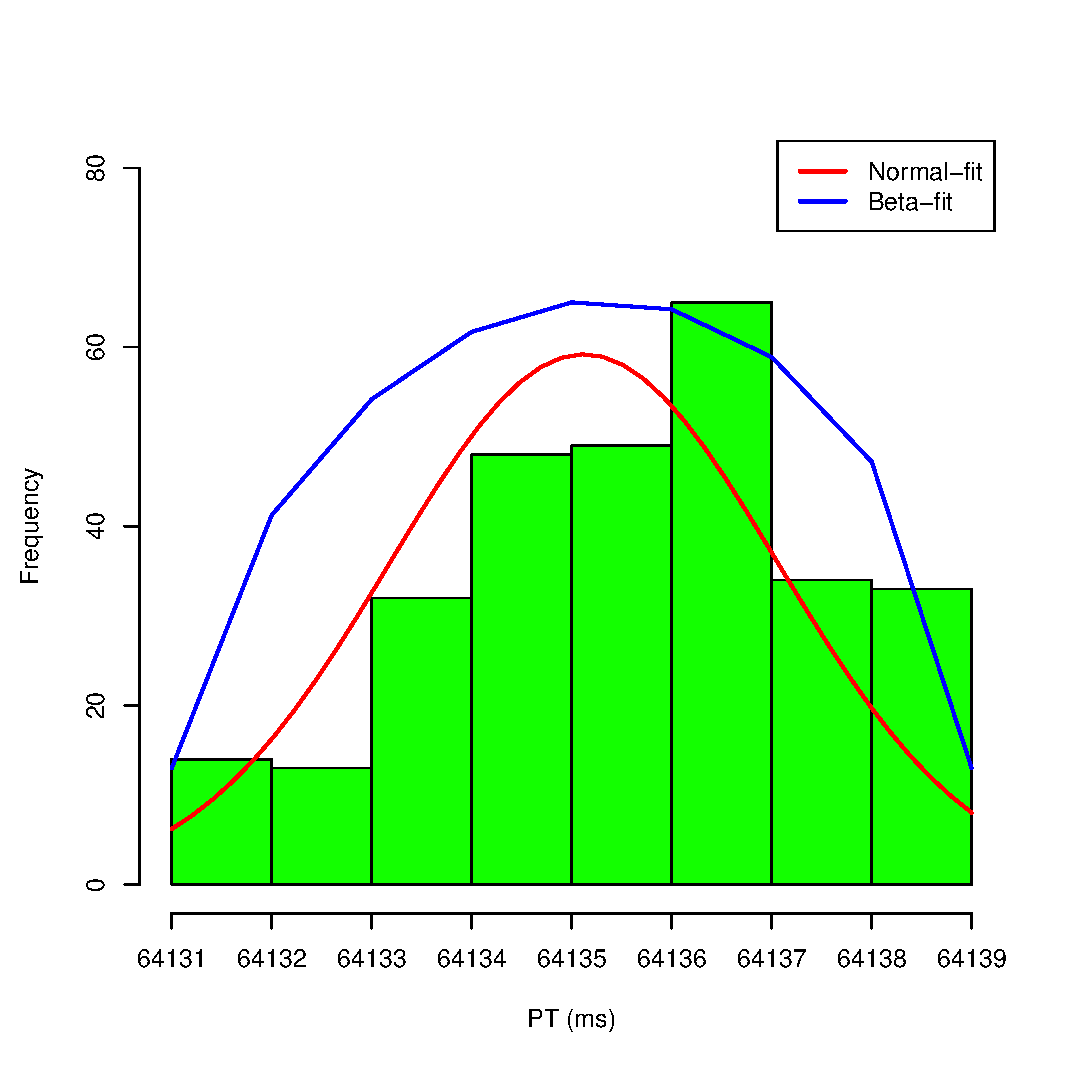
\includegraphics[scale=0.43]{figures/sodb12-ntp-on-turbo-off/64_sec_pt_hist.eps}
		\label{fig:64_sec_pt_hist1}
	}
	\subfigure[ET frequency on PUT128]{
		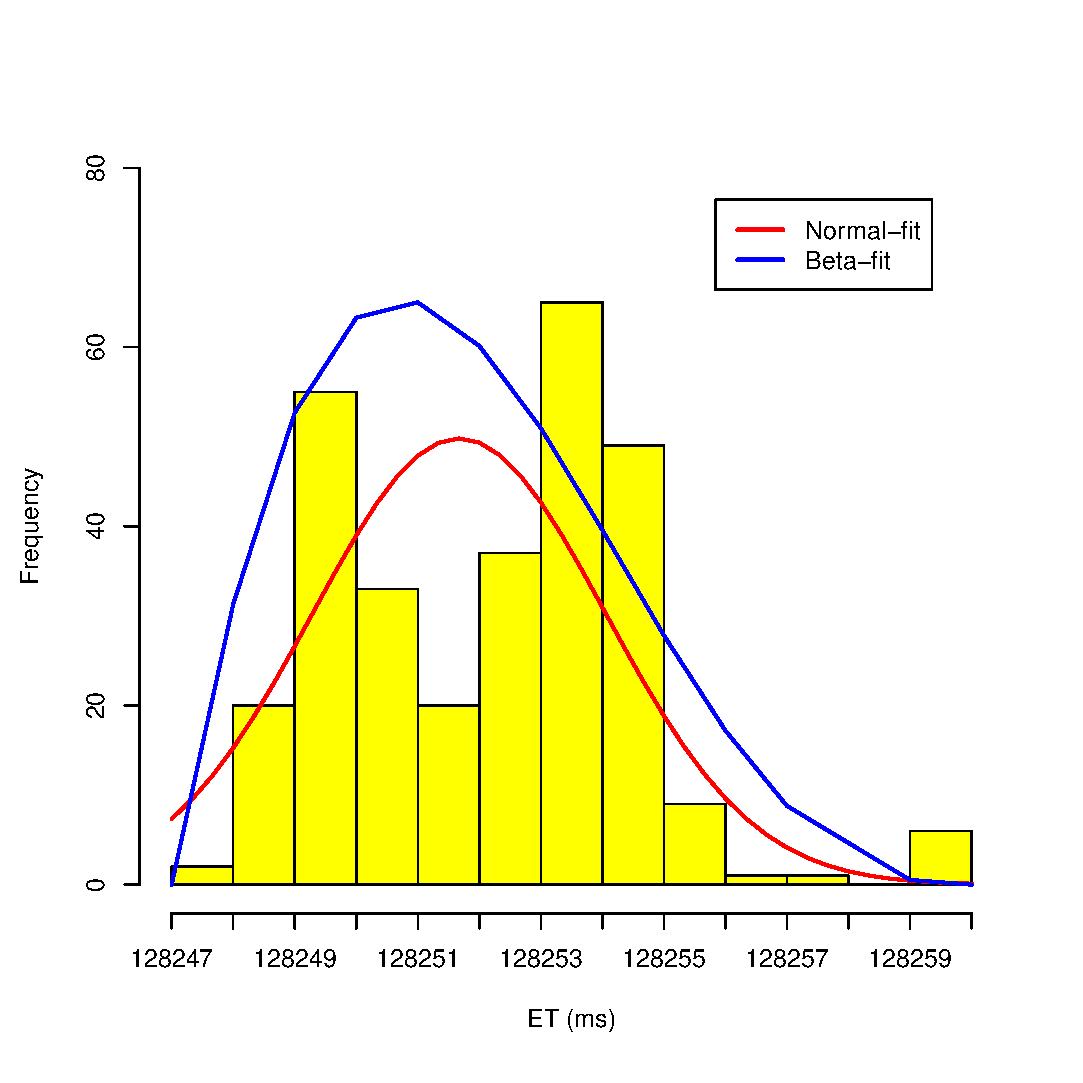
\includegraphics[scale=0.43]{figures/sodb12-ntp-on-turbo-off/128_sec_et_hist.eps}
		\label{fig:128_sec_et_hist1}
	}
	\subfigure[PT frequency on PUT128]{
		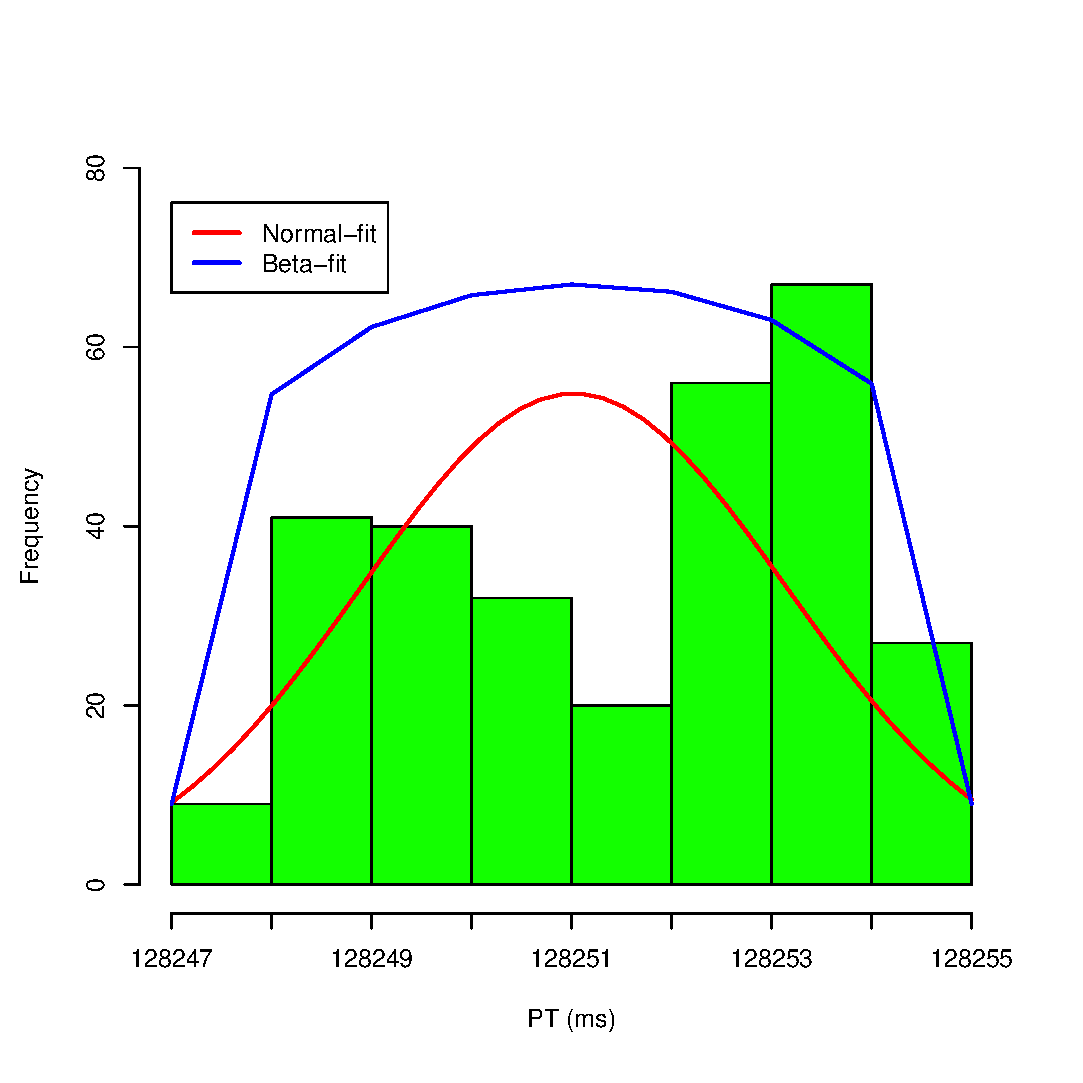
\includegraphics[scale=0.43]{figures/sodb12-ntp-on-turbo-off/128_sec_pt_hist.eps}
		\label{fig:128_sec_pt_hist1}
	}
	\caption{Normal and beta distributions fitting onto the histograms of the measurements of PUT64 and PUT128~\label{fig:extra_pt_hist4}}
\end{figure}

\begin{figure}[H]
	\centering
	\subfigure[ET frequency on PUT256]{
		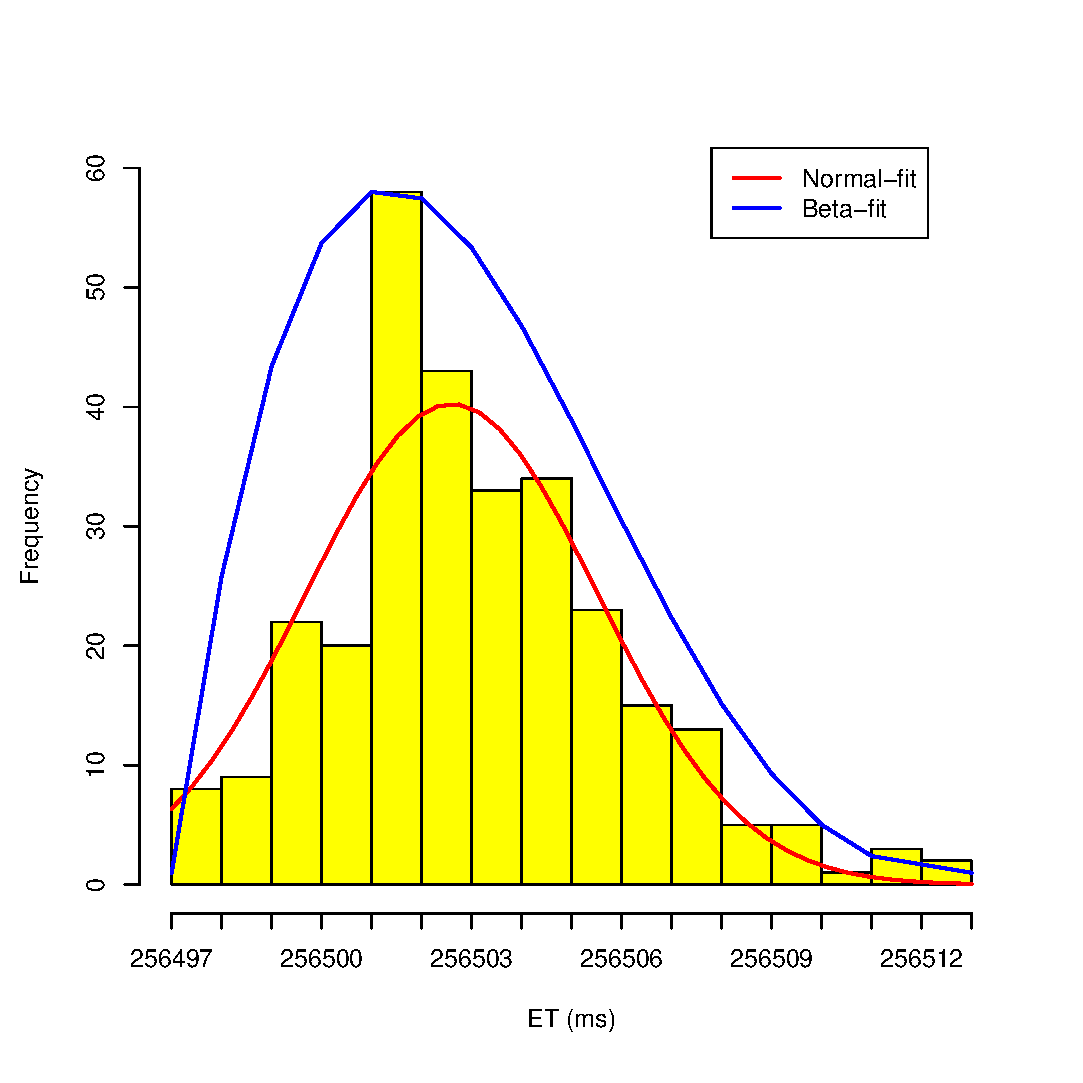
\includegraphics[scale=0.43]{figures/sodb12-ntp-on-turbo-off/256_sec_et_hist.eps}
		\label{fig:256_sec_et_hist1}
	}
	\subfigure[PT frequency on PUT256]{
		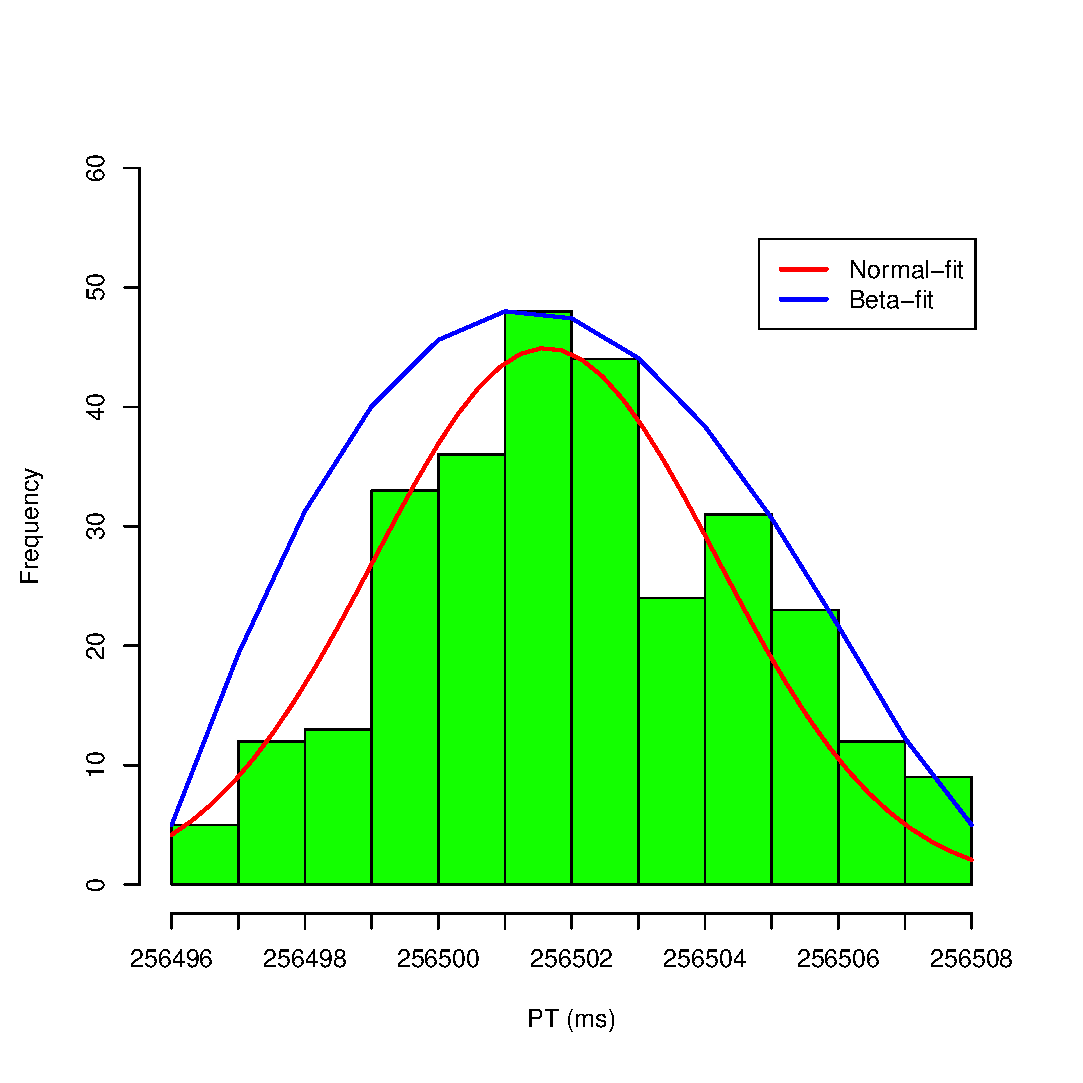
\includegraphics[scale=0.43]{figures/sodb12-ntp-on-turbo-off/256_sec_pt_hist.eps}
		\label{fig:256_sec_pt_hist1}
	}
	\subfigure[ET frequency on PUT512]{
		\includegraphics[scale=0.43]{figures/sodb12-ntp-on-turbo-off/512_sec_et_hist.eps}
		\label{fig:512_sec_et_hist1}
	}
	\subfigure[PT frequency on PUT512]{
		\includegraphics[scale=0.43]{figures/sodb12-ntp-on-turbo-off/512_sec_pt_hist.eps}
		\label{fig:512_sec_pt_hist1}
	}
	\caption{Normal and beta distributions fitting onto the histograms of the measurements of PUT256 and PUT512~\label{fig:extra_pt_hist5}}
\end{figure}

\begin{figure}[H]
	\centering
	\subfigure[ET frequency on PUT1024]{
		\includegraphics[scale=0.43]{figures/sodb12-ntp-on-turbo-off/1024_sec_et_hist.eps}
		\label{fig:1024_sec_et_hist1}
	}
	\subfigure[PT frequency on PUT1024]{
		\includegraphics[scale=0.43]{figures/sodb12-ntp-on-turbo-off/1024_sec_pt_hist.eps}
		\label{fig:1024_sec_pt_hist1}
	}
	\subfigure[ET frequency on PUT2048]{
		\includegraphics[scale=0.43]{figures/sodb12-ntp-on-turbo-off/2048_sec_et_hist.eps}
		\label{fig:2048_sec_et_hist1}
	}
	\subfigure[PT frequency on PUT2048]{
		\includegraphics[scale=0.43]{figures/sodb12-ntp-on-turbo-off/2048_sec_pt_hist.eps}
		\label{fig:2048_sec_pt_hist1}
	}
	\caption{Normal and beta distributions fitting onto the histograms of the measurements of PUT1024 and PUT2048~\label{fig:extra_pt_hist6}}
\end{figure}

\begin{figure}[H]
	\centering
		\subfigure[ET frequency on PUT4096]{
		\includegraphics[scale=0.43]{figures/sodb12-ntp-on-turbo-off/4096_sec_et_hist.eps}
		\label{fig:4096_sec_et_hist1}
	}
	\subfigure[PT frequency on PUT4096]{
		\includegraphics[scale=0.43]{figures/sodb12-ntp-on-turbo-off/4096_sec_pt_hist.eps}
		\label{fig:4096_sec_pt_hist1}
	}
	\caption{Normal and beta distributions fitting onto the histograms of the measurements of PUT4096~\label{fig:extra_pt_hist7}}
\end{figure}

\begin{figure}[H]
	\centering
		\subfigure[ET frequency on PUT8192]{
		\includegraphics[scale=0.43]{figures/sodb12-ntp-on-turbo-off/8192_sec_et_hist.eps}
		\label{fig:8192_sec_et_hist1}
	}
	\subfigure[PT frequency on PUT8192]{
		\includegraphics[scale=0.43]{figures/sodb12-ntp-on-turbo-off/8192_sec_pt_hist.eps}
		\label{fig:8192_sec_pt_hist1}
	}
	\caption{Normal and beta distributions fitting onto the histograms of the measurements of PUT8192~\label{fig:extra_pt_hist8}}
\end{figure}

\bibliographystyle{abbrv}
\newcommand{\etalchar}[1]{$^{#1}$}
\begin{thebibliography}{99}
\bibitem{Mills} David L. Mills, ``Internet Time Synchronization: The Network Time Protocol,'' in {\it IEEE Trans. on Comm.}, Vol. 39, No. 10, pp.~1482--1493, October, 1991.
\end{thebibliography}
\end{document}

